%% FEUP THESIS STYLE for LaTeX2e
%% how to use feupteses (English version)
%%
%% FEUP, JCL & JCF, 31 July 2012
%%
%% PLEASE send improvements to jlopes at fe.up.pt and to jcf at fe.up.pt
%%

%%========================================
%% Commands: pdflatex tese
%%           bibtex tese
%%           makeindex tese (only if creating an index) 
%%           pdflatex tese
%% Alternative:
%%          latexmk -pdf tese.tex
%%========================================

\documentclass[11pt,a4paper,twoside,openright]{report}

%% For iso-8859-1 (latin1), comment next line and uncomment the second line
\usepackage[utf8]{inputenc}
%\usepackage[latin1]{inputenc}

%% English version

%% MIEIC options
\usepackage[mieic]{feupteses}
%\usepackage[mieic,juri]{feupteses}
%\usepackage[mieic,final]{feupteses}
%\usepackage[mieic,final,onpaper]{feupteses}

%% Additional options for feupteses.sty: 
%% - onpaper: links are not shown (for paper versions)
%% - backrefs: include back references from bibliography to citation place

%% Uncomment the next lines if side by side graphics used
%\usepackage[lofdepth,lotdepth]{subfig}
%\usepackage{graphicx}
%\usepackage{float}

%% Include color package
\usepackage{color}
\definecolor{cloudwhite}{cmyk}{0,0,0,0.025}

%% Include source-code listings package
\usepackage{listings}
\lstset{ %
 language=C,                        % choose the language of the code
 basicstyle=\footnotesize\ttfamily,
 keywordstyle=\bfseries,
 numbers=left,                      % where to put the line-numbers
 numberstyle=\scriptsize\texttt,    % the size of the fonts that are used for the line-numbers
 stepnumber=1,                      % the step between two line-numbers. If it's 1 each line will be numbered
 numbersep=8pt,                     % how far the line-numbers are from the code
 frame=tb,
 float=htb,
 aboveskip=8mm,
 belowskip=4mm,
 backgroundcolor=\color{cloudwhite},
 showspaces=false,                  % show spaces adding particular underscores
 showstringspaces=false,            % underline spaces within strings
 showtabs=false,                    % show tabs within strings adding particular underscores
 tabsize=2,	                    % sets default tabsize to 2 spaces
 captionpos=b,                      % sets the caption-position to bottom
 breaklines=true,                   % sets automatic line breaking
 breakatwhitespace=false,           % sets if automatic breaks should only happen at whitespace
 escapeinside={\%*}{*)},            % if you want to add a comment within your code
 morekeywords={*,var,template,new}  % if you want to add more keywords to the set
}

\usepackage{rotating}
\usepackage{tikz}
\usetikzlibrary{matrix}
\usepackage{mathtools}
\usepackage{amsfonts}
\usepackage{algorithm}
\usepackage{algpseudocode}

%% Uncomment to create an index (at the end of the document)
%\makeindex

%% Path to the figures directory
%% TIP: use folder ``figures'' to keep all your figures
\graphicspath{{figures/}}

%%----------------------------------------
%% TIP: if you want to define more macros, use an external file to keep them
%some macro definitions

% format
\newcommand{\class}[1]{{\normalfont\slshape #1\/}}

% entities
\newcommand{\Feup}{Faculdade de Engenharia da Universidade do Porto}

\newcommand{\svg}{\class{SVG}}
\newcommand{\scada}{\class{SCADA}}
\newcommand{\scadadms}{\class{SCADA/DMS}}

% SWOT

\newcommand{\texta}{Helpful\\ \tiny (to achieve the objective)\par}
\newcommand{\textb}{Harmful\\ \tiny (to achieve the objective)\par}
\newcommand{\textcn}{Internal origin\\ \tiny (product\slash company attributes)\par}
\newcommand{\textdn}{External origin\\ \tiny (environment\slash market attributes)\par}

%%----------------------------------------

%%========================================
%% Start of document
%%========================================
\begin{document}

%%----------------------------------------
%% Information about the work
%%----------------------------------------
\title{Framework for Multi-Agent Simulation of User Behaviour in E-Commerce Sites}
\author{Duarte Duarte}

%% Uncomment next line for date of submission
\thesisdate{February 1, 2016}

%%Uncomment next line for copyright text if used
%\copyrightnotice{Name of the Author, 2008}

\supervisor{Supervisor}{Hugo Sereno Ferreira}

%% Uncomment next line if necessary
\supervisor{Second Supervisor}{João Azevedo}

%% Uncomment committee stuff in the final version if used
%\committeetext{Approved in oral examination by the committee:}
%\committeemember{Chair}{Doctor Name of the President}
%\committeemember{External Examiner}{Doctor Name of the Examiner}
%\committeemember{Supervisor}{Doctor Name of the Supervisor}
%\signature

%% Specify cover logo (in folder ``figures'')
\logo{uporto-feup.pdf}

%% Uncomment next line for additional text  below the author's name (front page)
\additionalfronttext{Dissertation Planning}

%%----------------------------------------
%% Preliminary materials
%%----------------------------------------

% remove unnecssary \include{} commands
\begin{Prolog}
  \chapter*{Abstract}

% TODO Rewrite, same as initial summary

Customers interact with e-commerce websites in multiple ways and the
companies operating them rely on optimizing success metrics for profit. 
Changing what, how and when content such as product recommendations and ads are 
displayed can influence customers' actions.

Multiple algorithms and techniques in data mining and machine learning
have been applied in this context. Summarizing and analysing user
behaviour can be expensive and tricky since it's hard to extrapolate
patterns that never occurred before and the causality aspects of the
system are not usually taken into consideration. Commonly used online
techniques have the downside of having a high operational cost. However, there 
has been studies about characterizing user behaviour and interactions in 
e-commerce websites that could be used to improve this process.

The goal of this dissertation is to create a framework capable of running
a multi-agent simulation, by regarding users in an e-commerce website that
react to stimuli that influence their actions. By taking input from web mining, 
which includes both static and dynamic content of websites as well as user 
personas, the simulation should collect success metrics so that the 
experimentation being run can be evaluated.

\chapter*{Resumo}

Consumidores interagem com websites de comércio eletrónico de várias formas e 
as empresas que os operam dependem da otimização de métricas de sucesso tais 
como \textit{CTR} (\textit{Click through Rate}), \textit{CPC} (\textit{Cost per 
Conversion}), \textit{Basket} e \textit{Lifetime Value} e \textit{User 
Engagement} para lucro. Alterar como, onde e quando o conteúdo de páginas web 
como por exemplo recomendação de produtos e publicidade é mostrado pode 
influenciar as ações dos consumidores.

Vários algoritmos e técnicas em \textit{data mining} e \textit{machine 
learning} têm sido aplicados neste contexto. Sumarizar e analisar comportamento 
de utilizadores pode ser custoso e complicado porque é difícil extrapolar 
padrões que nunca ocorreram antes e os aspetos causais do sistema geralmente 
não são tidos em consideração. Técnicas \textit{online} geralmente usadas têm o 
problema de ter um custo operacional elevado. Porém, existem estudos sobre 
caracterizar comportamento e interações de utilizadores em sites de comércio 
eletrónico que podem ser usados para melhorar este processo.

O objetivo desta dissertação é criar uma \textit{framework} capaz de correr uma 
simulação multi-agente, tendo em conta os utilizadores de um site de comércio 
eletrónico que reagem a estímulos que influenciam as suas ações. Extraindo 
dados de web mining, que inclui tanto conteúdo estático como dinâmico de 
websites assim como de perfis de utilizadores, a simulação deve reportar 
métricas de sucesso para que a experiência possa ser avaliada.
 % the abstract
  % \chapter*{Acknowledgements}

Aliquam id dui. Nulla facilisi. Nullam ligula nunc, viverra a, iaculis
at, faucibus quis, sapien. Cum sociis natoque penatibus et magnis dis
parturient montes, nascetur ridiculus mus. Curabitur magna ligula,
ornare luctus, aliquam non, aliquet at, tortor. Donec iaculis nulla
sed eros. Sed felis. Nam lobortis libero. Pellentesque
odio. Suspendisse potenti. Morbi imperdiet rhoncus magna. Morbi
vestibulum interdum turpis. Pellentesque varius. Morbi nulla urna,
euismod in, molestie ac, placerat in, orci. 

Ut convallis. Suspendisse luctus pharetra sem. Sed sit amet mi in diam
luctus suscipit. Nulla facilisi. Integer commodo, turpis et semper
auctor, nisl ligula vestibulum erat, sed tempor lacus nibh at
turpis. Quisque vestibulum pulvinar justo. Class aptent taciti
sociosqu ad litora torquent per conubia nostra, per inceptos
himenaeos. Nam sed tellus vel tortor hendrerit pulvinar. Phasellus
eleifend, augue at mattis tincidunt, lorem lorem sodales arcu, id
volutpat risus est id neque. Phasellus egestas ante. Nam porttitor
justo sit amet urna. Suspendisse ligula nunc, mollis ac, elementum
non, venenatis ut, mauris. Mauris augue risus, tempus scelerisque,
rutrum quis, hendrerit at, nunc. Nulla posuere porta orci. Nulla dui. 

Fusce gravida placerat sem. Aenean ipsum diam, pharetra vitae, ornare
et, semper sit amet, nibh. Nam id tellus. Etiam ultrices. Praesent
gravida. Aliquam nec sapien. Morbi sagittis vulputate dolor. Donec
sapien lorem, laoreet egestas, pellentesque euismod, porta at,
sapien. Integer vitae lacus id dui convallis blandit. Mauris non
sem. Integer in velit eget lorem scelerisque vehicula. Etiam tincidunt
turpis ac nunc. Pellentesque a justo. Mauris faucibus quam id
eros. Cras pharetra. Fusce rutrum vulputate lorem. Cras pretium magna
in nisl. Integer ornare dui non pede. 

\vspace{10mm}
\flushleft{The Name of the Author}
  % the acknowledgments
  % \cleardoublepage
\thispagestyle{plain}

\vspace*{8cm}

\begin{flushright}
   \textsl{``You should be glad that bridge fell down. \\
           I was planning to build thirteen more to that same design''} \\
\vspace*{1.5cm}
           Isambard Kingdom Brunel
\end{flushright}
       % initial quotation if desired
  \cleardoublepage
  \pdfbookmark[0]{Table of Contents}{contents}
  \tableofcontents
  \cleardoublepage
  \pdfbookmark[0]{List of Figures}{figures}
  \listoffigures
  \cleardoublepage
  \pdfbookmark[0]{List of Tables}{tables}
  \listoftables
  \chapter*{Abbreviations}
\chaptermark{ABBREVIATIONS}

\begin{flushleft}
\begin{tabular}{l p{0.8\linewidth}}
% TODO order me
ABS      & Agent Based Simulation\\
API      & Application Programming Interface\\
CBMG     & Customer behavior model graph\\
CPC      & Cost per Conversion\\
CTR      & Click through Rate\\
DAG      & Directed acyclic graph\\
DES      & Discrete Event Simulation\\
HMM      & Hidden Markov model\\
JPD      & Joint probability distribution\\
LTV      & Lifetime Value\\
MOOC     & Massive Open Online Course\\
PGM      & Probabilistic Graphical Model\\
SD       & System Dynamics\\
SWOT     & Strengths, Weaknesses, Opportunities and Threats\\
WCM      & Web content mining\\
WSM      & Web structure mining\\
WUM      & Web usage mining\\
WWW      & \emph{World Wide Web}
\end{tabular}
\end{flushleft}
  % the list of abbreviations used
\end{Prolog}

%%----------------------------------------
%% Body
%%----------------------------------------
\StartBody

%% TIP: use a separate file for each chapter
\chapter{Introdução} \label{chap:intro}

\section*{}

O primeiro capítulo da dissertação deve servir para apresentar o
enquadramento e a moti\-va\-ção do trabalho e para identificar e
definir os problemas que a dissertação aborda.
Deve resumir as metodologias utilizadas no trabalho e termina
apresentando um breve resumo de cada um dos capítulos
posteriores.

Este documento ilustra o formato a usar em dissertações na \Feup, não
servindo de exemplo sobre os conteúdos a usar.
São dados exemplos de margens, cabeçalhos, títulos, paginação, estilos
de índices, etc. 
São ainda dados exemplos de formatação de citações, figuras e tabelas,
equações, referências cruzadas, lista de referências e índices.

Uma recolha de normas existentes sobre este assunto pode ser
encontrada em~\cite{kn:Mat93}. 

\begin{quote}
  ``Like the Abstract, the Introduction should be written to engage the
  interest of the reader. It should also give the reader an idea of
  how the dissertation is structured, and in doing so, define the
  thread of the contents.''~\cite[chap.\ Introduction]{kn:Tha01} 
\end{quote}

Neste primeiro capítulo ilustra-se a utilização de citações e de
referências biblio\-grá\-fi\-cas.
Para além de dar um exemplo de utilização de uma citação, a citação
anterior, introduz uma referência que pode ser consultada, entre
muitas outras referências bibliográficas
interessantes~\cite{kn:Tha01,kn:PP05}. 

\section{Contexto/Enquadramento} \label{sec:context}

Esta secção descreve a área em que o trabalho se insere, podendo
referir um eventual projeto de que faz parte e apresentar uma breve
descrição da empresa onde o trabalho decorreu.

Lorem ipsum~\cite{kn:Lip08} dolor sit amet, consectetuer adipiscing
elit. 
Sed eget nunc. Phasellus interdum, risus viverra mollis laoreet, felis
justo iaculis ante, eget ornare purus augue non urna. Nam in magna. In a
est. Phasellus a tellus vitae enim vehicula imperdiet. Etiam sit amet
elit. In hac habitasse platea dictumst. Quisque eget turpis vel felis
elementum tempus. Curabitur sit amet tortor id libero dapibus
pretium. Integer mattis eros eu lorem. Duis erat tellus, porttitor
sed, blandit eget, fringilla et, lacus. Phasellus tristique nibh nec
orci. Mauris sed leo. Suspendisse fringilla tempor dolor. Donec sapien
enim, congue in, porta et, sollicitudin in, quam. Curabitur semper,
mauris ut vestibulum eleifend, diam ipsum tincidunt quam, et
vestibulum velit mauris ut risus. 

Sed eget libero. Nulla facilisi. Proin eget tortor. Morbi
gravida. Donec arcu risus, blandit a, rutrum at, ornare ut,
nisl. Etiam consectetuer tortor eu odio. Etiam blandit molestie
ligula. Nulla facilisi. Nam a augue non justo laoreet hendrerit. Nam
aliquam, purus eu ultricies dictum, urna purus posuere neque, vel
tempus tellus enim a arcu. 

\section{Projeto} \label{sec:proj}

Na continuação da secção anterior, e apenas no caso de ser um Projeto
e não uma Dissertação, esta secção apresenta resumidamente o projeto.

Nulla nec eros et pede vehicula aliquam. Aenean sodales pede vel
ante. Fusce sollicitudin sodales lacus. Maecenas justo mauris,
adipiscing vitae, ornare quis, convallis nec, eros. Etiam laoreet
venenatis ipsum. In tellus odio, eleifend ac, ultrices vel, lobortis
sed, nibh. Fusce nunc augue, dictum non, pulvinar sed, consectetuer
eu, ipsum. Vivamus nec pede. Pellentesque pulvinar fringilla dolor. In
sit amet pede. Proin orci justo, semper vel, vulputate quis, convallis
ac, nulla. Nulla at justo. Mauris feugiat dolor. Etiam posuere
fermentum eros. Morbi nisl ipsum, tempus id, ornare quis, mattis id,
dolor. Aenean molestie metus suscipit dolor. Aliquam id lectus sed
nisl lobortis rhoncus. Curabitur vitae diam sed sem aliquet
tempus. Sed scelerisque nisi nec sem. 

\section{Motivação e Objetivos} \label{sec:goals}

Apresenta a motivação e enumera os objetivos do trabalho terminando
com um resumo das metodologias para a prossecução dos objetivos.

Lorem ipsum dolor sit amet, consectetuer adipiscing elit. Morbi sit
amet nibh. Fusce faucibus, enim vel ultrices ornare, est mauris
ultricies velit, vitae consequat sem erat vel nunc. Nam libero eros,
mattis eget, sagittis nec, imperdiet at, sapien. Aliquam lacus. Aenean
adipiscing nibh in orci. Aliquam vestibulum, elit at fringilla
dignissim, metus diam lobortis urna, a laoreet nunc odio ac ipsum. Sed
at urna. Integer vehicula fringilla augue. Nulla lacus eros, rhoncus
sit amet, posuere ut, vehicula ac, nibh. Ut eleifend, eros eu placerat
vehicula, justo turpis blandit dolor, eu tincidunt felis risus at
ante. Aenean suscipit nisl eget eros. Ut laoreet libero eget
enim. Cras tempus pellentesque felis. Vestibulum vitae erat ac nibh
posuere eleifend. 

Integer nec quam. Sed fermentum. Nunc vitae leo. Etiam sit amet
quam. Nunc vestibulum massa in mauris. Duis eget nulla. Fusce
ultricies arcu eu nibh volutpat feugiat. Maecenas urna pede, commodo
quis, porta eu, bibendum elementum, pede. Sed eros massa, molestie
eget, mattis non, rutrum ac, magna. Duis dui. Maecenas eget tortor ut
dolor semper mattis. Maecenas auctor, tellus et ultricies tempor, elit
est placerat lacus, in posuere mauris lorem et arcu. 

\section{Estrutura da Dissertação} \label{sec:struct}

Para além da introdução, esta dissertação contém mais x capítulos.
No capítulo~\ref{chap:sota}, é descrito o estado da arte e são
apresentados trabalhos relacionados. 
%\todoline{Complete the document structure.}
No capítulo~\ref{chap:chap3}, ipsum dolor sit amet, consectetuer
adipiscing elit.
No capítulo~\ref{chap:chap4} praesent sit amet sem. 
No capítulo~\ref{chap:concl}  posuere, ante non tristique
consectetuer, dui elit scelerisque augue, eu vehicula nibh nisi ac
est. 
 % intro
\chapter{E-commerce background} \label{chap:ecommerce}

\section*{}

In this chapter we discuss some key concepts related to e-commerce, for the 
purpose of giving context to the dissertation. We discuss the typical customer 
life cycle in an e-commerce website, some metrics that might be used and some 
ways on how the customer interaction with the website might be influenced and 
improved.

\section{Introduction}

E-commerce, or electronic commerce, can be described by the trading of products 
or services over the Internet (or other computer networks). The type of 
e-commerce businesses we are interested are those who sell their goods directly 
to the customer, e.g online shopping, using an online store or catalog of 
products. Some popular online 
stores\footnote{\url{http://www.alexa.com/topsites/category/Top/Shopping}} are 
Amazon\footnote{\url{http://www.amazon.com/}}, 
Ebay\footnote{\url{http://www.ebay.com/}} and 
Alibaba\footnote{\url{http://www.alibaba.com/}}.

\section{Customer life cycle}

An important concept to understand the customer is by describing its life 
cycle, as presented by~\cite[Section 6]{Sterne2000} in 
figure~\ref{fig:lifecycle}.

\begin{figure}[h]
  \begin{center}
    \leavevmode
    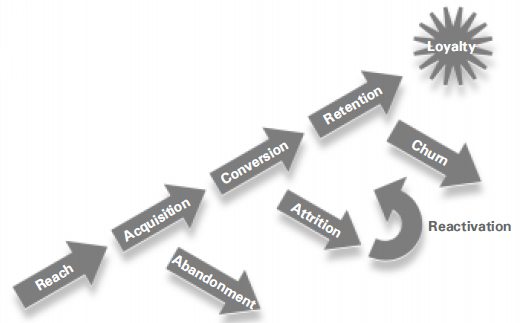
\includegraphics[width=0.86\textwidth]{lifecycle}
    \caption{Customer lifecycle \cite{Sterne2000}}
    \label{fig:lifecycle}
  \end{center}
\end{figure}

It starts by reaching the target audience or market up to an established 
customer base, not forgetting about those that drop mid way, due to abandonment 
or attrition.

\begin{itemize}
    \item Reach happens outside of the website and refers to the number of 
    potential customers. For example, if the online store is advertised on a 
    social network, the reach is the number of users who were served the ad in 
    that other website, they may or may not ignore it.
    \item Acquisition is the next stage, where the user decides to act on and 
    visits the website (or some other action like subscribing to a newsletter).
    \item Conversion is the stage where a visitor stops being a user and starts 
    being a customer. It usually means that the user made a purchase but some 
    companies might consider a sign up or registration in the website as a 
    conversion.
    \item Retention focuses on making existing customers, that made at least 
    one purchase before, repeat purchases.
    \item Loyalty is a stronger form of retention, which represents a greater 
    trust level of the customer in the store.
    \item Abandonment is defined by the customers that started the buying 
    process but do not finish it. For example, a customer may add items to the 
    online shopping cart but instead of moving to the next step, e.g. enter 
    credit card details, they exit the website or go elsewhere. This may happen 
    in any store with a multi-step buying process, which is very common.
    \item Attrition happens when a retained customer ceases buying from the 
    store and starts using a competitor store.
    \item Churn is defined by the number of customer that attrited during a 
    certain period divided by the total number of customers at the end of that 
    period. It measures how much of the customer base "rolls over" in a certain 
    time period.
\end{itemize}

\section{Customer Behavior Model Graph (CBMG)}

A state transition graph named Customer Behavior Model Graph (CBMG) can be used 
to describe the behaviour of customers browsing a website. The nodes represent 
the possible states or pages, e.g home page, product page, search, and a 
probability is associated with each transition. An example of such a CBMG is 
shown in figure \ref{fig:cbmg}.

\begin{figure}[h]
    \begin{center}
        \leavevmode
        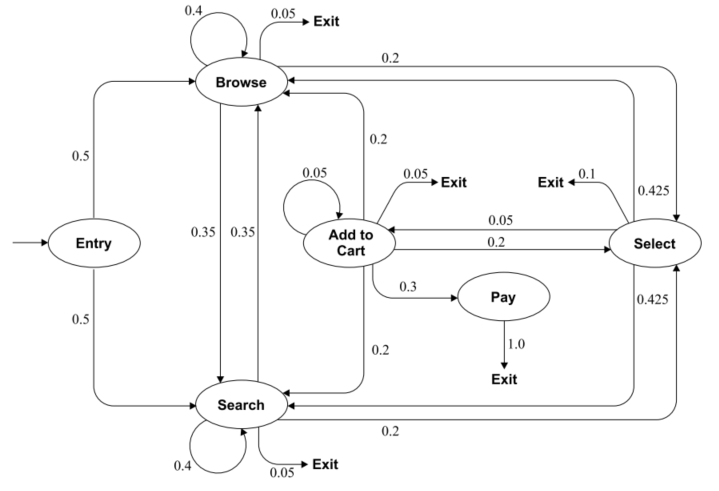
\includegraphics[width=0.86\textwidth]{cbmg}
        \caption{Example of a customer behaviour model graph \cite{Menasce1999}}
        \label{fig:cbmg}
    \end{center}
\end{figure}

\cite{Menasce1999} describes how CBMGs can be used to analyse the workload of 
an e-commerce store server and how metrics can be derived directly from the 
CBMG alone.

\section{E-commerce metrics}

Metrics are a common way to quantify, measure, benchmark or evaluate some 
process. In an e-commerce setting, businesses are interested in optimizing, 
mostly, for profit. Different businesses prioritize metrics in different ways, 
adapted to each use case. Here we present some common used metrics, but this 
list is by no means exhaustive. \cite{Sterne2000, Menasce1999}

\begin{itemize}
    \item \textit{Conversion Rate} (CR) is the percentage of visitors that buy 
    a product or a service;
    \item \textit{Shopping Cart Abandonment} is the percentage of visitors that 
    added a product to the online cart but did not complete the process;
    \item \textit{Average Order Value} (AOV) is the average size of an order;
    \item \textit{Customer Lifetime Value} (LTV) is the projected value that a 
    customer will spend on the store;
    \item \textit{Clicks to Buy} (CTB) is the average number of clicks a 
    visitor has to do to complete a buy order;
    \item \textit{Churn Rate} the percentage of customers that do not make a 
    repeated purchase;
    \item \textit{Bounce Rate} is the percentage of visitors that arrive at the 
    homepage of the online store but leave immediately, without clicking 
    anything or visiting a different page.
\end{itemize}

There are other common metrics such as \textit{Acquisition Cost}, \textit{Cost 
Per Conversion}, \textit{Net Yield} or \textit{Connection Rate} however they 
are associated with promotion campaigns that happen outside of the store 
website, therefore they are not interesting in the context of our work.

\section{Influencing user behaviour}

Tracking a bunch of statistics and metrics about an online store is no good if 
there are no actionable changes that can be done using that information. 
\cite{Constantinides2004} describes functionality, psychological and content 
factors that can influence the visitor experience, represented in the table 
\ref{tab:factors}.

\begin{table}[h]
    \centering
    \caption{Main building blocks of Web experience and their sub-categories 
    \cite{Constantinides2004}}
\label{tab:factors}
\begin{tabular}{lll}
    \cline{1-2}
    \multicolumn{2}{|c|}{\textbf{Functionality 
    factors}}                                               & 
    \textbf{}                                   \\ \cline{1-2}
    \multicolumn{1}{|l|}{\textbf{Usability}}             & 
    \multicolumn{1}{l|}{\textbf{Interactivity}} & 
    \textbf{}                                   \\ \cline{1-2}
    Convenience                                          & Customer 
    service/after sales                
    &                                             \\
    Site navigation                                      & Interaction with 
    company personnel          &                                             \\
    Information architecture                             & 
    Customization                               &                               
                  \\
    Ordering/payment process                             & Network 
    effects                             &                                       
          \\
    Search facilities and process                        
    &                                             &                             
                    \\
    Site speed                                           
    &                                             &                             
                    \\
    Findability/accessibility                            
    &                                             &                             
                    \\
    &                                             
    &                                             \\ \hline
    \multicolumn{1}{|l|}{\textbf{Psychological factors}} & 
    \multicolumn{2}{c|}{\textbf{Content 
    factors}}                                             \\ \hline
    \multicolumn{1}{|l|}{\textbf{Trust}}                 & 
    \multicolumn{1}{l|}{\textbf{Aesthetics}}    & 
    \multicolumn{1}{l|}{\textbf{Marketing mix}} \\ \hline
    Transaction security                                 & 
    Design                                      & 
    Communication                               \\
    Customer data misuse                                 & Presentation 
    quality                        & 
    Product                                     \\
    Customer data safety                                 & Design 
    elements                             & 
    Fulfillment                                 \\
    Uncertainty reducing elements                        & 
    Style/atmosphere                            & 
    Price                                       \\
    Guarantees/return policies                           
    &                                             & 
    Promotion                                   \\
    &                                             & 
    Characteristics                            
\end{tabular}
\end{table}

Regarding usability of the online store, providing a personalized experience to 
each customer can be very beneficial for both the customer and the business. A 
common way to do this is by recommending products that the customer might be 
interested it \cite{Adomavicius2005}. For example, if we know that a customer 
buys mostly football related products, recommending her more products in the 
same category might increase sales.

\section{Summary}

In this chapter we covered a brief overview of e-commerce, starting with the 
customer lifecycle, how to measure it using metrics and presenting a common way 
to model the users' behaviour, the CBMG.
 % state of the art: e-commerce
\chapter{Implementation} \label{chap:implementation}

\section*{}

\todo{intro}

\section{Methodology} \label{sec:meth}

Like any software development project, a simulation project also has a life 
cycle. In this section we describe the steps to apply in the simulation 
methodology, based on Ulgen et al.~\cite{Ulgen1994} and Banks et 
al.~\cite[section 1.11]{Banks2004}, which can be summarized as follows:

\begin{enumerate}
    \item \textit{Problem formulation}: Clear statement of the problem by the 
    analyst and stakeholders; \label{enum:mform}
    \item \textit{Setting of objectives and overall project plan}: Questions to 
    be answered by the simulation, plans for the study, cost and number of days 
    for each phase, with the results expected at each stage; \label{enum:mobj}
    \item \textit{Model conceptualization}: Select, modify and iterate over the 
    assumptions that characterize the system; \label{enum:mconcept}
    \item \textit{Data collection}: Collect the necessary data to run and 
    validate the model, assuming that required data will change with the 
    increasing complexity of the system; \label{enum:mdata}
    \item \textit{Model translation}: Materialization of the system in a 
    program; \label{enum:mtransl}
    \item \textit{Verification}: Making sure that the program behaves correctly 
    accordingly to its inputs; \label{enum:mverif}
    \item \textit{Validation}: Calibration of the model, comparing the model 
    against an actual system; \label{enum:mvalid}
    \item \textit{Experimental design}: Tweak the experiments, comparing 
    alternative designs; \label{enum:mexp}
    \item \textit{Production runs and analysis}: Estimate measures of 
    performance for the systems that are being simulated; \label{enum:mprod}
    \item \textit{Documentation and reporting}: Document both the program and 
    the progress of the study; \label{enum:mdocs}
    \item \textit{Implementation}: End result of the study, including the 
    entire simulation process. \label{enum:mimpl}
\end{enumerate}

This process can be visualized in figure \ref{fig:sim}.

\begin{figure}[p]
    \begin{center}
        \leavevmode
        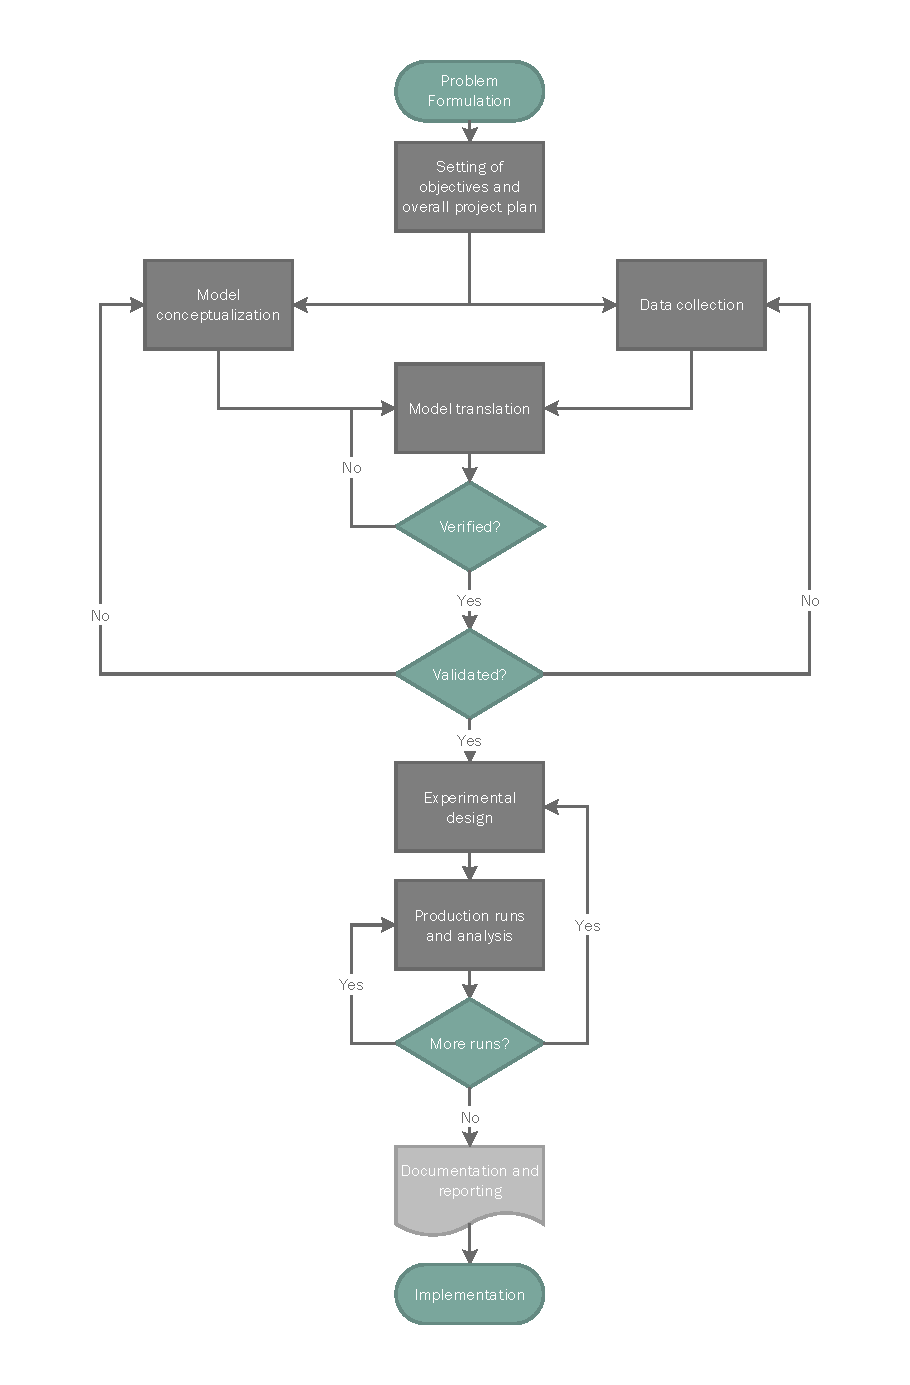
\includegraphics[width=0.95\textwidth]{simulation_study}
        \caption{Steps in a simulation study \cite{Banks2004}}
        \label{fig:sim}
    \end{center}
\end{figure}

\section{Requirements}

\subsection{Website Representation}
\subsection{Navigation Agents}
\subsection{Website Agents}
\subsection{Simulation Engine}
\subsection{Reporting}

\section{Architecture}

\subsection{Multi-agent Architecture}

The simulation framework encompasses two different kinds of agents, navigation 
agents and website agents, as shown in figure \ref{fig:agent_arch}.

\begin{figure}[h]
    \begin{center}
        \leavevmode
        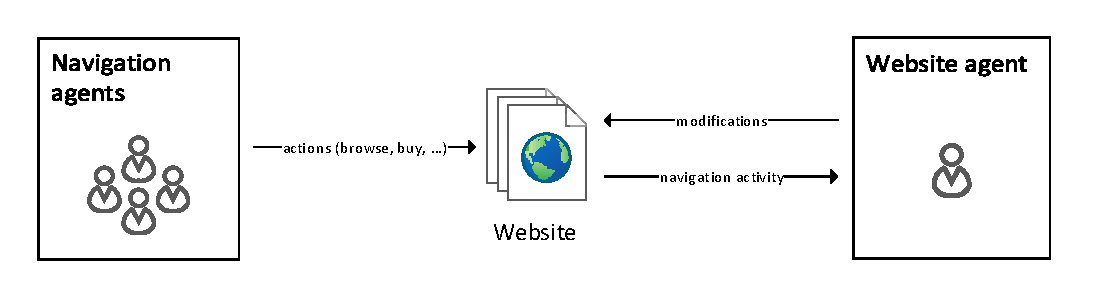
\includegraphics[width=0.95\textwidth]{agent_architecture}
        \caption{Agent architecture}
        \label{fig:agent_arch}
    \end{center}
\end{figure}

Navigation agents represent users interacting with the website. They have a 
limited view of the system: they have access to the website (pages and links 
between them) and they know the current page they are visiting. Each simulation 
step, the framework asks each navigation agent which action will they pick. The 
action may be to visit another page (\texttt{BrowseToAction}), exit the 
website (\texttt{ExitAction}), add a product to the cart 
(\texttt{AddToCartAction}), finish the purchase (\texttt{CheckoutAction}) 
or simply do nothing (\texttt{IdleAction}). Also related to the navigation 
agents subsystem, an implementation of \texttt{NavigationAgentFactory} is 
used to decide how many navigation agents are added to the system in each step. 
For example, a simplistic implementation might create a fixed number of 
navigation agents or a different one closer to reality could follow a Poisson 
distribution model \cite{gunduz2003poisson}.

% LIMITATION & future work: limited/hardcoded number of actions

Website agents are able to modify the pages before they are served to the 
users. They have a broader view of the system than navigation agents. They are 
notified of all the actions that the navigation agents do. The most common use 
case of the website agents is to recommend products to the users: before the 
page is served to a user, a website agent can modify a section of the page to 
display a custom list of products, based on the previous activity of the other 
users or preferences of the current user. However they are not limited to only 
recommendations, a website agent might replace a page's content entirely, 
increase or decrease the price of products (e.g promotions, sales), do nothing, 
etc.

The framework does not assume how these agents behave however the interactions 
between them are limited. The agents do not send messages between each other 
and may only interact indirectly, through the framework (e.g a website agent 
modifies a page before it is "seen" by a navigation agent). While a simulation 
run might have hundreds or thousands of navigation agents, to simplify, each 
run only has one website agent instance (this does not impose a limit on the 
solution, the agent can still be modelled after a composite agent\footnote{An 
    agent that represents multiple composite or virtual agents (our name)}).

It is out of the scope of the framework to provide concrete implementations of 
the agents but we provide 2 implementations of navigation agents and 3 
implementations of website agents, as a way to validate and verify the 
simulation runs. This will be further discussed in 
chapter~\ref{chap:validation}.

\subsection{Simulation Engine}

The simulation engine follows a fairly standard and simple discrete event 
simulation architecture, as described in \ref{ssec:des}. The domain model we 
are dealing with allows certain simplifications of the simulation:

\begin{itemize}
    \item the event list only contains events scheduled for the next step;
    \item there are no conditional events (type C \cite{pidd1998computer});
    \item all the events happen instantaneously;
    \item the events do not depend on other events, they do not require 
    synchronization and may be implemented in a single-threaded engine.
\end{itemize}

The process that the simulation engine is described next. In each simulation 
loop, the engine starts by calling \textproc{newNavigationAgents()} which adds 
new navigation agents to the simulation. The number and type of these agents 
are decided by the \texttt{NavigationAgentFactory}. After that, each 
navigation agent currently active (i.e did not leave the website) chooses an 
action to do (buy, browse, etc., defined below). Depending on the action that 
was picked, the engine updates its internal state. The simulation state is 
represented by \texttt{WebsiteState} and contains statistics and other 
performance metrics. Whenever the picked action implies presenting the 
navigation agent a page from the website, the website agent can modify that 
page before it is presented, by calling \textproc{modifyPage(navAgent, page)}. 
The website agent is also notified about all actions that the navigation agents 
do (\textproc{notify(navAgent, action)}). The simulation is configured to end 
after a fixed number of steps, otherwise it could run forever.

This process is illustrated in figure \ref{fig:sequence_diagram}. 

\begin{figure}[h]
    \begin{center}
        \leavevmode
        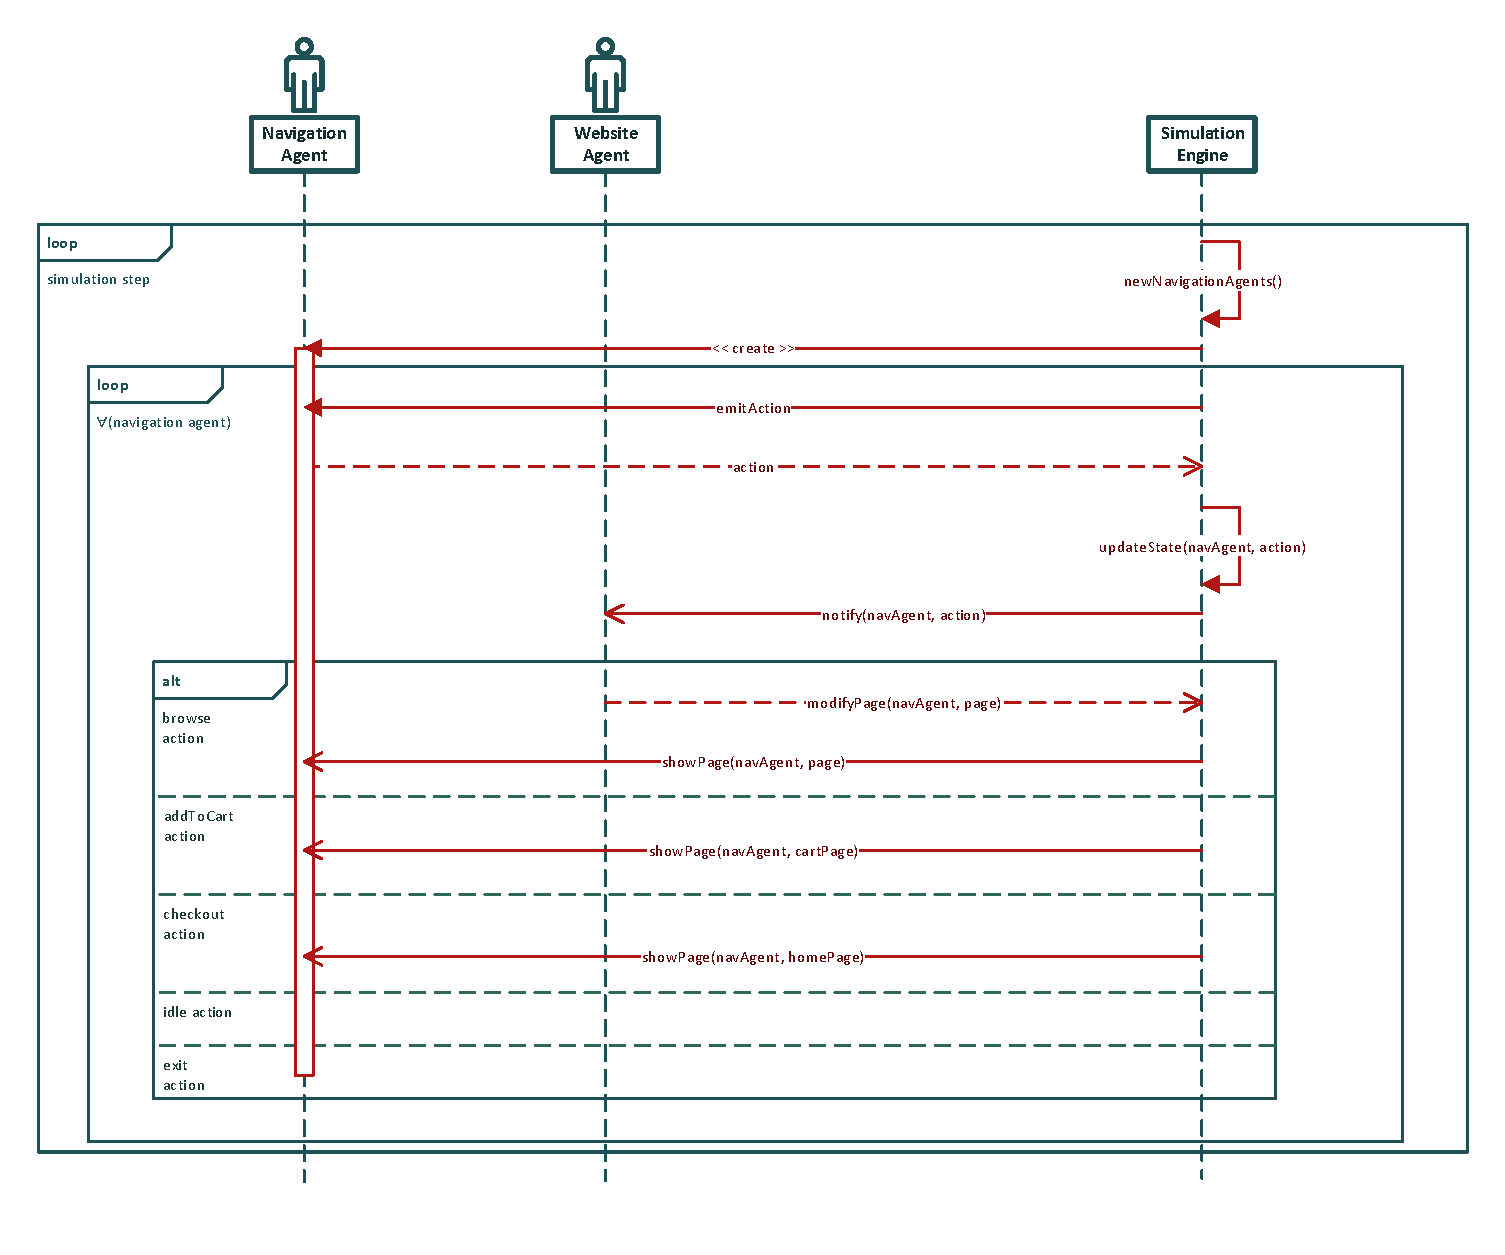
\includegraphics[width=0.95\textwidth]{sequence_diagram}
        \caption{Sequence diagram for the simulation engine}
        \label{fig:sequence_diagram}
    \end{center}
\end{figure}

\subsection{Class Model}

In this sub-section we describe all the classes used to represent all the 
entities in the simulation engine (figure \ref{fig:class}).

\texttt{Website} represents a website, it contains a set of \texttt{pages} and 
a reference to its \texttt{homepage}, the entry point of the website. A 
\texttt{Page} has a set of \texttt{links}, which are all the outbound 
hyperlinks that a page contains, it has a set of \texttt{tags}, which is used 
to categorize a page (e.g electronics category, clothing category, cart page, 
product search page, etc.) and the page may also contain a \texttt{Product}, if 
the page is a product page. A \texttt{Product} has a \texttt{name}, a 
\texttt{description} and a \texttt{price}.

The \texttt{Simulation} is an abstract class that contains an \texttt{agenda} 
which stores all the \texttt{Action}s (an arbitrary function) to be executed in 
the next steps, it provides a way to enqueue work in the simulation using 
\textproc{schedule(delay, action)} and a \textproc{run()} method that consumes 
the \texttt{agenda} until there's no more work to do. A subclass of 
\texttt{Simulation}, \texttt{WebsiteSimulation} represents a simulation 
happening over websites. It contains the \texttt{Website} itself, a 
\texttt{WebsiteState}, a \texttt{NavigationUserFactory} and a 
\texttt{WebsiteAgent}. The \texttt{WebsiteState} is used to keep track of all 
the statistics and metrics that the simulation produces. This state can be 
stored in a database to analyse the results once the simulation is finished.

\texttt{NavigationAgent} is an interface that represents users interacting with 
the website. Implementations of it have to implement \textproc{emitAction}, 
which returns the \texttt{Action} the agents wants to do based on their 
internal state and their current page. These agents are added to the simulation 
by an implementation of \texttt{NavigationAgentFactory}. \texttt{WebsiteAgent} 
is an interface that represents the agents that may modify the website and that 
are notified about all the navigation agent activity.

The mutability of the system is contained to the \texttt{Simulation} (due to 
its \texttt{agenda}) and \texttt{WebsiteState} which is updated every 
simulation step.

The points of extensibility of the framework are the agents interfaces 
(\texttt{NavigationAgent}, \texttt{NavigationAgentFactory} and 
\texttt{WebsiteAgent}) and \texttt{WebsiteState} (e.g provide additional 
tracking metrics or visualizations).

\begin{figure}[p]
    \begin{center}
        \leavevmode
        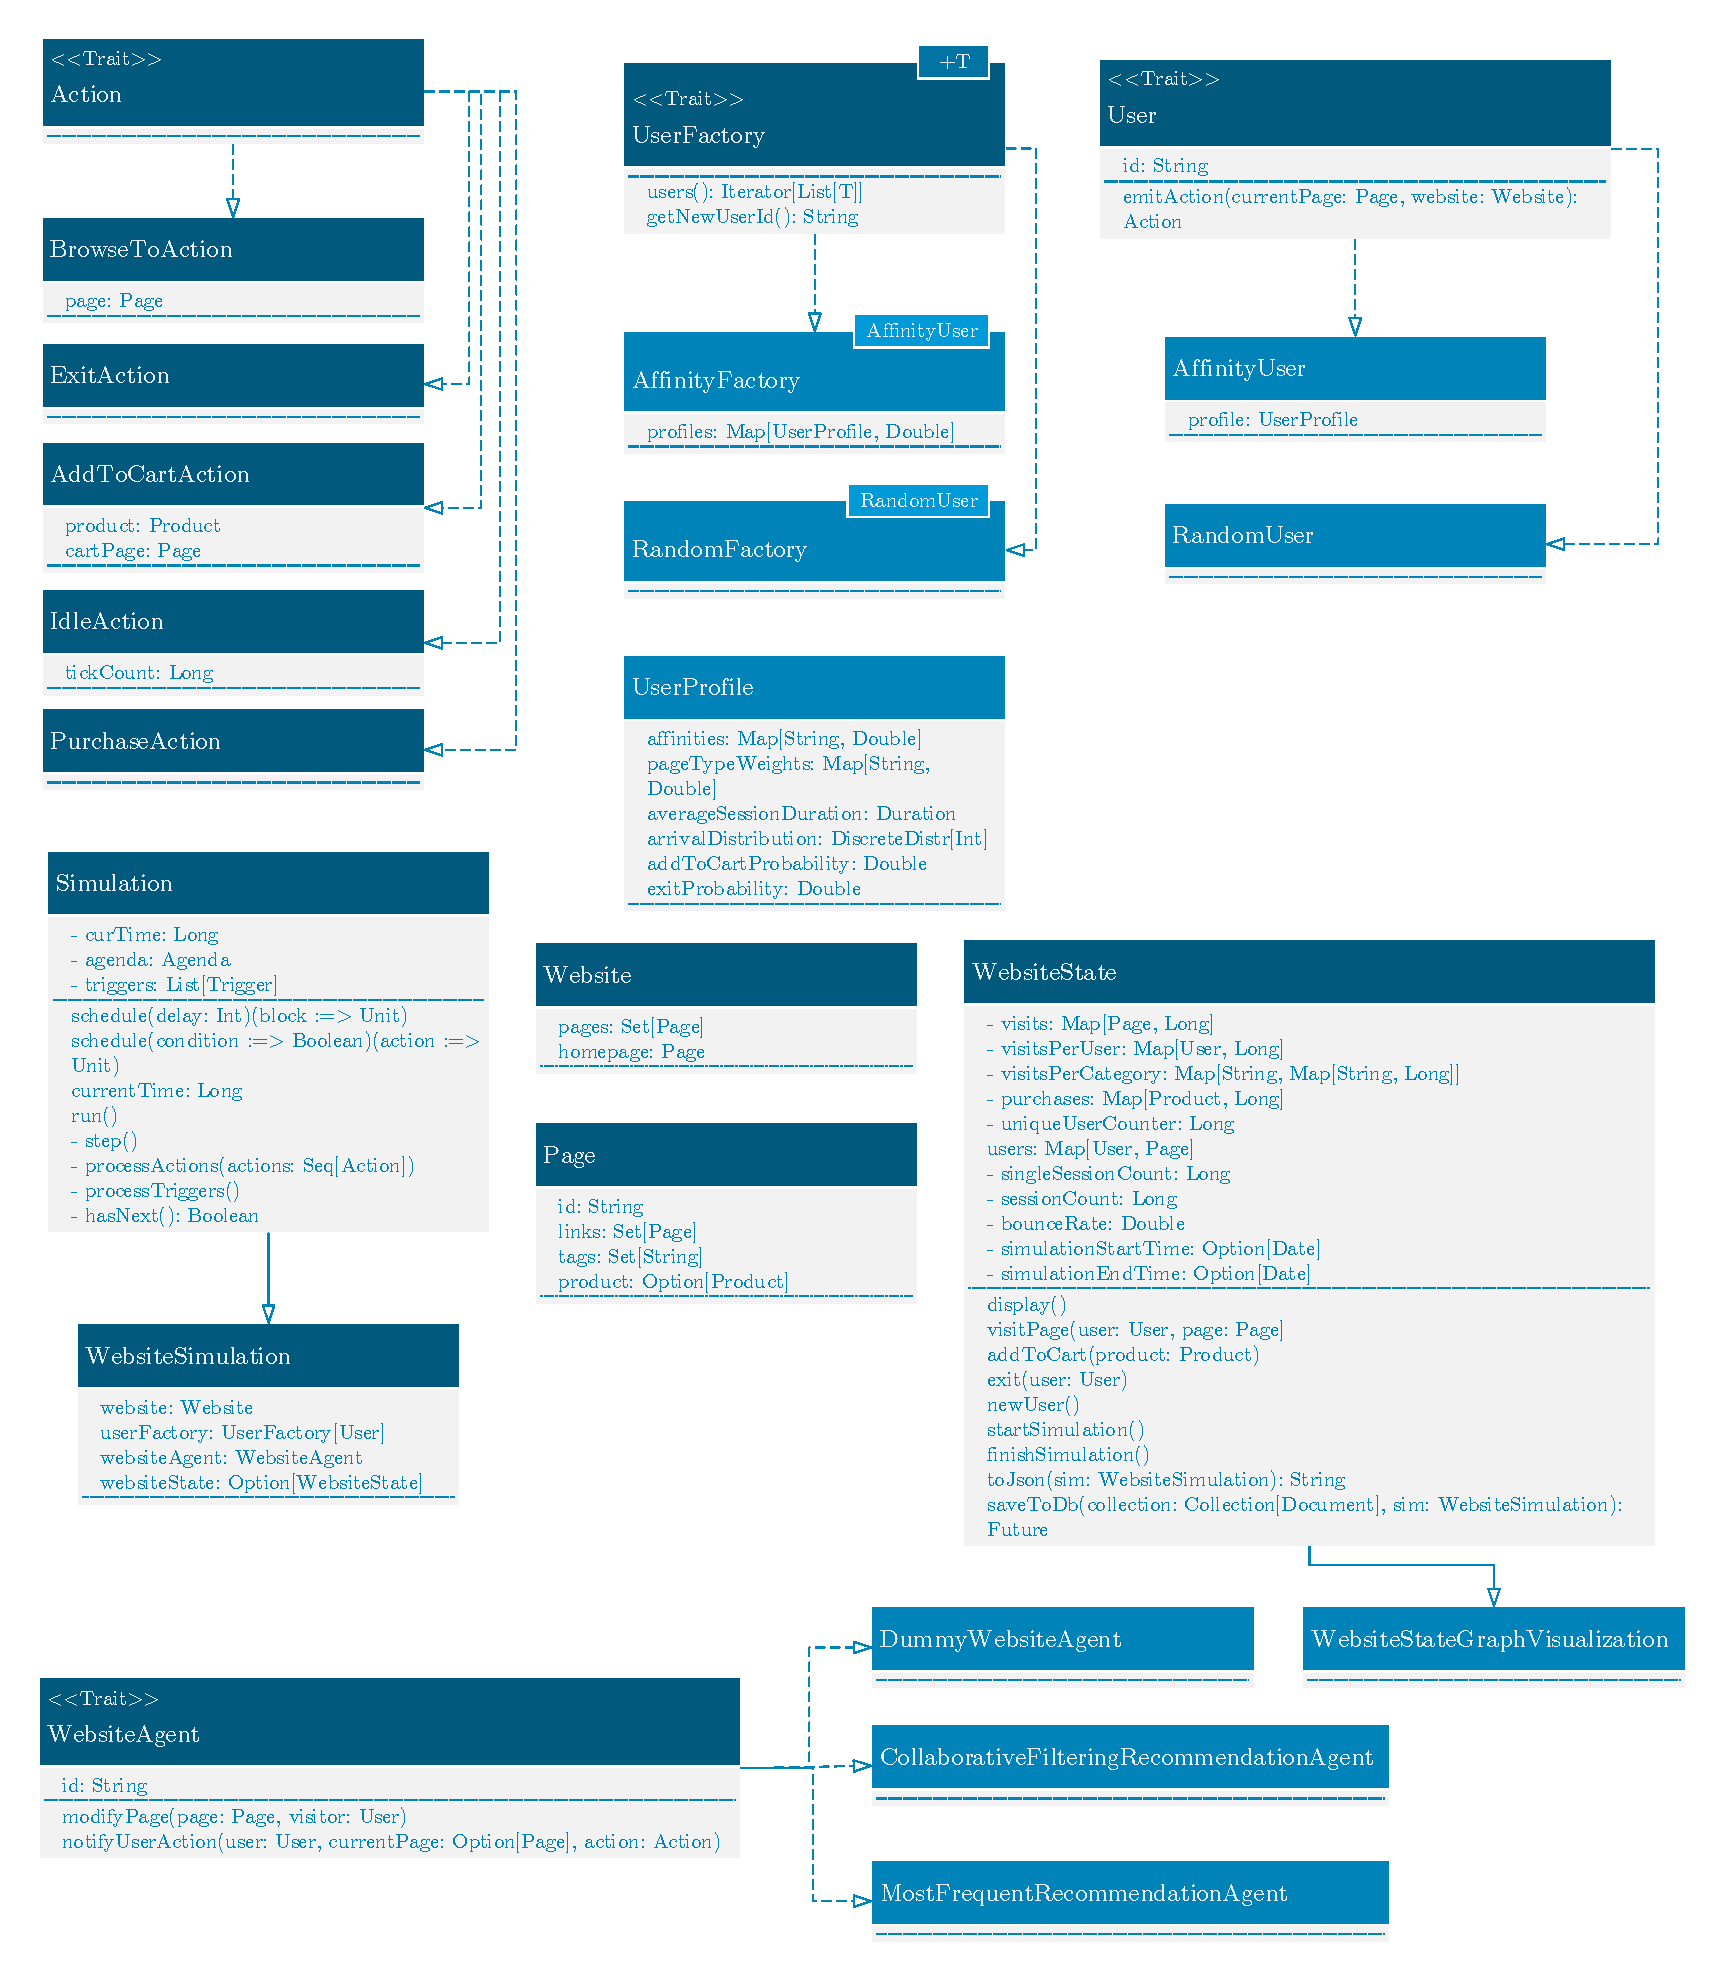
\includegraphics[width=0.95\textwidth]{class_diagram}
        \caption{Class diagram}
        \label{fig:class}
    \end{center}
\end{figure}

\subsection{Graphical User Interface}

A frontend website has been developed to aid in displaying and visualizing the 
results of each simulation run. The data is loaded asynchronously from a 
database which stores \texttt{WebsiteState} snapshots. All the data is rendered 
to the user server-site except the data required to display charts (e.g Visits 
per Category chart).

The interface has three distinct views: a simulation list, details about a 
simulation run and comparison between two simulation runs:

\begin{itemize}
    \item The simulation list view (\texttt{\textbf{GET} /simulations}) (figure 
    \ref{fig:sim_view}) displays a table 
    with all the simulation runs stored in the database. It shows the 
    identifier, name, agent types and timestamp of each run.
    \item The detail view (\texttt{\textbf{GET} /simulations/\textit{<id>}}) 
    (figure \ref{fig:sim_detail_view})
    display information regarding a single simulation run. This info describes 
    the simulation and it contains data regarding the types of the agents used, 
    start and finish time of the simulation, collected metrics (e.g bounce 
    rate, conversion rate, total order value, etc.), visits per page, visits 
    per page category, purchases per product and others. This information is 
    displayed using mostly tables and charts.
    \item The last view, the comparison page (\texttt{\textbf{GET} 
    /simulations/compare/\textit{<idA>}/\textit{<idB>}}) (figure 
    \ref{fig:sim_compare_view}) displays information 
    regarding two simulation runs (A and B) side by side, so they can be 
    compared and analysed. The planned use case of this view is to quickly spot 
    differences between two runs and see how different agent configurations 
    affect the results.
\end{itemize}


\section{Scalability}

To assess the scalability and performance of the simulation engine, some 
benchmarks were made and they are described next. The tests were ran in a 
Windows 10 laptop with a Intel\textregistered~Core\texttrademark~i7-4710HQ CPU 
@ 2.50GHz (8 CPUs) processor. A modified\footnote{Changed each measurement to 
run the same block of code 10 times, drop the first 2 runs and take the average 
of the 8 runs instead of running it only once.} version of the library 
Benchmark.scala\footnote{\url{https://github.com/balagez/Benchmark.scala}} was 
used, which is based on Ruby's Benchmark 
module\footnote{\url{http://ruby-doc.org/stdlib-1.9.2/libdoc/benchmark/rdoc/Benchmark.html}}.
 The focus is not necessarily in the raw speed of the engine but rather in the 
variation of the simulation time when the number of agents in the system or the 
number of steps of the simulation are increased.

The test performed consists of running the same simulation with an 
increasing number of navigation agents and number of simulation steps, set up 
in the following way:

\begin{itemize}
    \item \textbf{Website}: Toy sample website with 9 pages and 32 total links 
    between pages (1 homepage, 1 cart page, 3 product list pages and 4 product 
    pages);
    \item \textbf{Website agent}: Dummy agent, does not modify any page;
    \item \textbf{Navigation agent}: Sample agent implementation which 
    picks the next action randomly. Configured with a chance of exiting the 
    website of $\frac{1}{3}$ and a change of adding a product to the cart of 
    $\frac{1}{20}$;
    \item \textbf{Number of navigation agents}: From 1000 to 10000 with 
    increments of 1000;
    \item \textbf{Number of simulation steps}: From 100 to 1000 with increments 
    of 100.
\end{itemize}

The result of the 100 simulation runs is shown in figure \ref{fig:simbench} 
(whose data is in table \ref{tab:simbench}). A quick analysis shows that the 
simulation time scales linearly ($\bar{R^{2}} = 0.99149, \sigma = 0.00648$) 
with both the number of agents and the number of simulation steps. For 
instance, a simulation with 1000 steps and 10000 navigation agents (entering 
the system each step)	 took 41.95 seconds. These initial results are very 
satisfactory however they should be improved, especially when the number of 
steps is increased, so that simulations that span a longer period of time can 
be evaluated (e.g simulate the effect of seasonal consumers over an entire 
year).

\begin{figure}[h]
    \begin{center}
        \leavevmode
        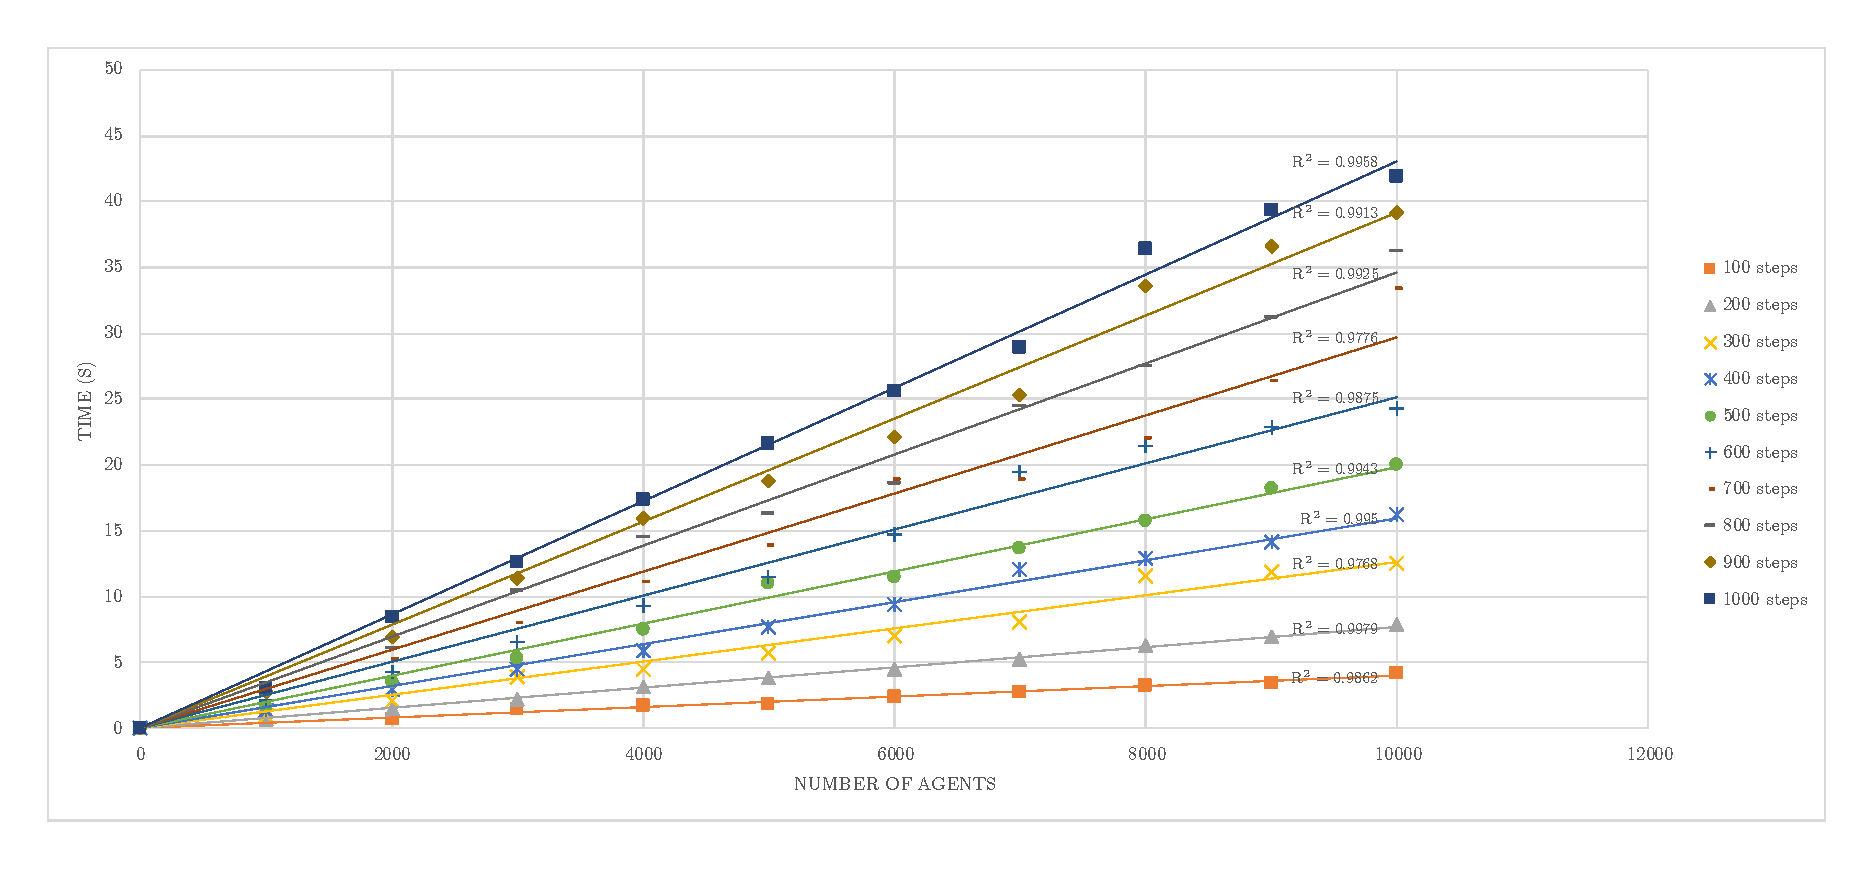
\includegraphics[width=0.95\textwidth]{simulation_benchmark}
        \caption{Simulation running time for different number of 
        navigation agents and simulation steps}
        \label{fig:simbench}
    \end{center}
\end{figure}

\begin{table}[h]
    \centering
    \caption{Simulation running time (in seconds) for different number of 
    navigation agents and simulation steps}
    \label{tab:simbench}
    \begin{tabular}{@{}lllllllllll@{}}
        \toprule
        \diaghead(5, -3){Stepagent}{Steps}{Agents} & 1000 & 2000 & 3000 & 4000 
        & 5000 
        & 
        6000 & 7000 & 8000 & 
        9000 & 10000 \\ \midrule
        100 & 0.62 & 0.69 & 1.45 & 1.72 & 1.81 & 2.34 & 2.76 & 3.23 & 3.42 & 
        4.16 \\
        200 & 0.67 & 1.43 & 2.20 & 3.17 & 3.84 & 4.49 & 5.22 & 6.30 & 6.93 & 
        7.89 \\
        300 & 0.95 & 2.07 & 3.90 & 4.44 & 5.72 & 7.01 & 8.05 & 11.62 & 11.89 & 
        12.53 \\
        400 & 1.32 & 2.91 & 4.42 & 5.88 & 7.69 & 9.39 & 12.01 & 12.93 & 14.15 & 
        16.18 \\
        500 & 1.58 & 3.48 & 5.34 & 7.49 & 11.03 & 11.44 & 13.65 & 15.77 & 18.20 
        & 20.00 \\
        600 & 2.10 & 4.31 & 6.59 & 9.26 & 11.52 & 14.71 & 19.44 & 21.47 & 22.83 
        & 24.29 \\
        700 & 2.55 & 5.24 & 7.97 & 11.14 & 13.89 & 18.91 & 18.89 & 22.04 & 
        26.33 & 33.35 \\
        800 & 2.56 & 6.10 & 10.46 & 14.48 & 16.31 & 18.56 & 24.49 & 27.52 & 
        31.19 & 36.26 \\
        900 & 2.77 & 6.94 & 11.37 & 15.97 & 18.77 & 22.11 & 25.36 & 33.56 & 
        36.57 & 39.21 \\
        1000 & 3.07 & 8.47 & 12.64 & 17.40 & 21.59 & 25.62 & 28.94 & 36.46 & 
        39.40 & 41.95 \\ \bottomrule
    \end{tabular}
\end{table}

\todo{More tests?}

\section{Technology}
 % state of the art: simulation
\chapter{Validation} \label{chap:validation}

\section*{}

% To validate the framework 3 testbeds were prepared. The first is a collection 
% of small fabricated test cases where we compare the output of multiple 
% simulation runs to the expected results. The second and third cases deal with 
% real uses of the framework, applied in two different e-commerce contexts: the 
% first is an online store of computer products and the second is a general 
% comparison shopping website.

To validate the framework 2 testbeds were prepared. The first is a collection 
of small fabricated test cases where we compare the output of multiple 
simulation runs to the expected results. The second case deals with a real use 
of the framework, applied to an online store.

% \section{Validation methodology}

\section{Sanity checks} % rename?

\subsection{Expected number of agents in the simulation}

This test compares the number of navigation agents expected to be 
\textit{alive} at each simulation step with the actual number of them.

At each simulation step, $k$ navigation agents enter the system and  
$p_{exit}$ of them leaves, which leads to the recurrence equation \ref{eq:recc}.

\begin{equation}\label{eq:recc}
\begin{cases}
a_{1} = \left (1 - p_{exit}  \right ) k\\
a_{n} = \left (1 - p_{exit}  \right ) \left (k + a_{n - 1} \right)
\end{cases} \Leftrightarrow a_{n} = \frac{k (p_{exit}-1) ((1-p_{exit})^{n} - 
1)}{p_{exit}}
\end{equation}

The simulation run was configured in the following way:

\begin{itemize}
    \item \textbf{Website}: Sample website with 9 pages and 32 total links 
    between pages
    \item \textbf{Website agent}: Dummy agent, does not modify any page;
    \item \textbf{Navigation agent}: Sample agent implementation with a chance 
    of exiting the website of $\frac{1}{3}$ ($p_{exit}$);
    \item \textbf{Number of new navigation agents each step}: 100 ($k$)
    \item \textbf{Number of simulation steps}: 1000
\end{itemize}

Replacing the values in equation \ref{eq:recc}: $a_{n} = -200 \left ( 
\frac{2}{3}^{n} - 1 \right )$. After a few simulation runs, the expected number 
of agents in the system stabilizes: $\lim_{n\to \infty} -200 \left ( 
\frac{2}{3}^{n} - 1 \right ) = 200$.

The results of a simulation run were gathered and plotted in figure 
\ref{fig:expagents}. Triangles ($\triangle$) represent the actual value 
($A_{t}$) and circles ($\bullet$) represent the expected value ($E_{t}$) 
according to the equations above. SMAPE (symmetric mean absolute percentage 
error)\cite{makridakis1993accuracy} is used to measure the accuracy of the 
results: $ SMAPE = {\frac {1}{n}}\sum _{t=1}^{n}{\frac 
{\left|E_{t}-A_{t}\right|}{|A_{t}|+|E_{t}|}} = 3.07\% $, which is a reasonable 
low \textit{error} rate given the randomness of the system.

\begin{figure}[h]
    \begin{center}
        \leavevmode
        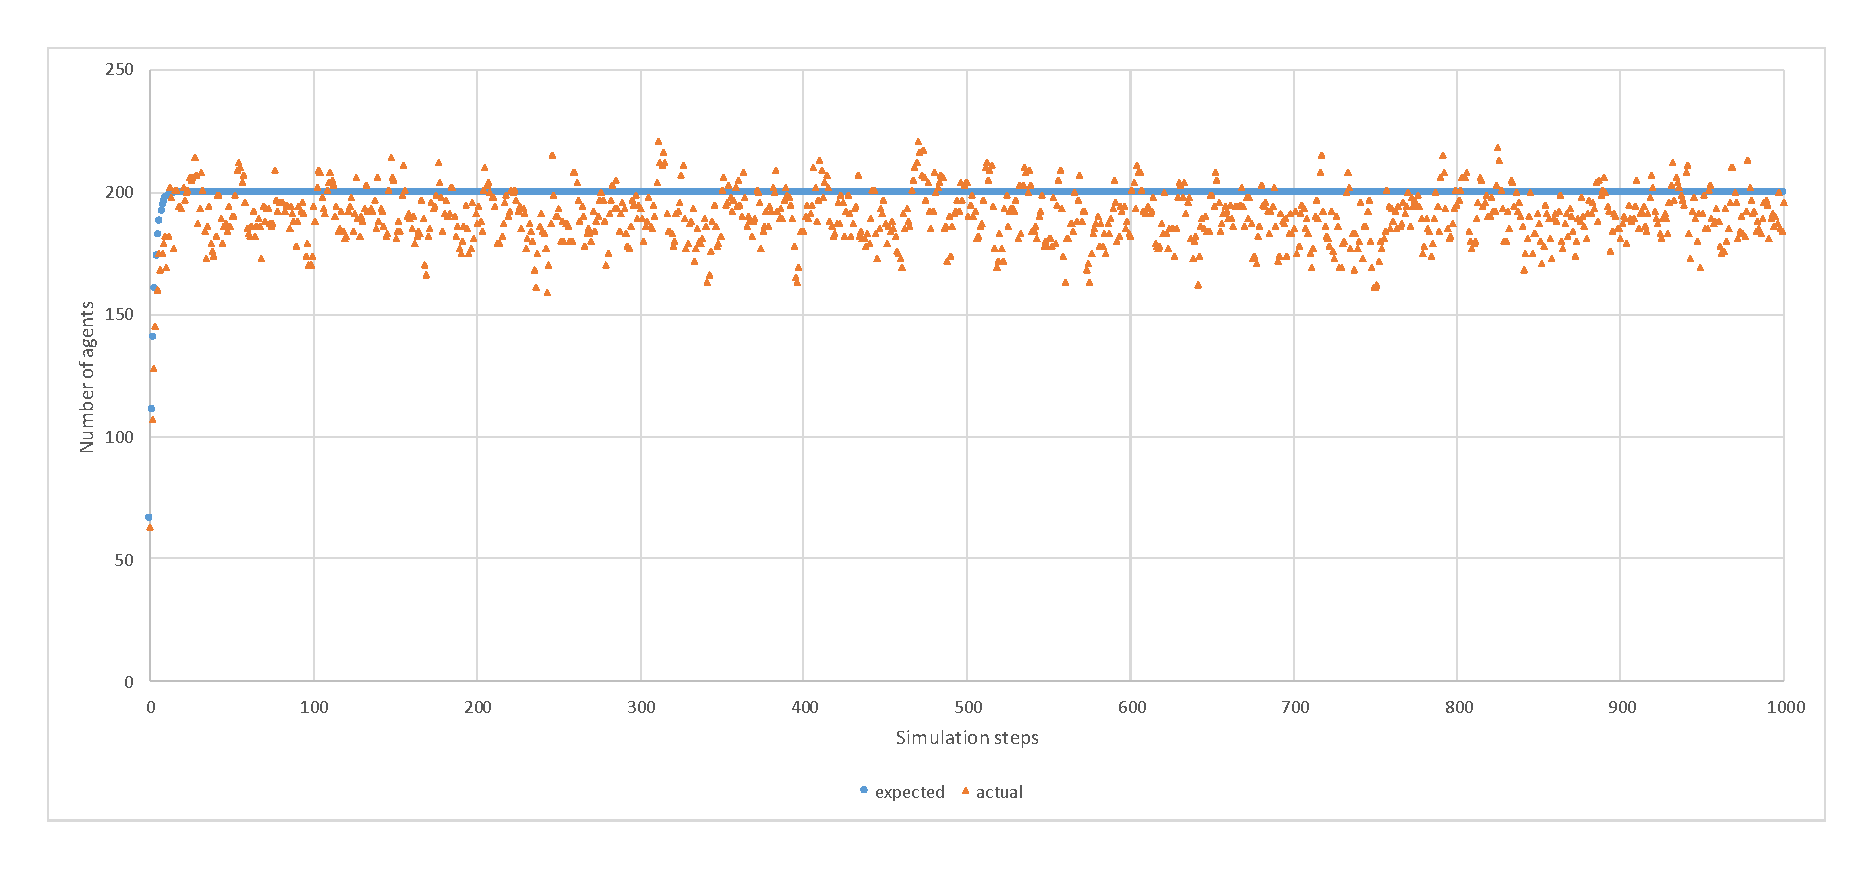
\includegraphics[width=1\textwidth]{expected_agents}
        \caption{Expected number of agents in the simulation}
        \label{fig:expagents}
    \end{center}
\end{figure}

\subsection{Expected number of visits}

This test compares the number of visits (page hits) for a given website and 
agents setup. The simulation run was configured in the following way:

\begin{itemize}
    \item \textbf{Website}: Website configured as displayed in figure 
    \ref{fig:test2website}. The homepage links to 5 product pages and the 
    product page link to the cart page.
    \item \textbf{Website agent}: Dummy agent, does not modify any page;
    \item \textbf{Navigation agent}: The agent picks one linked page randomly, 
    however, if current page is for a product, it always buys it. If the 
    current page is the cart page, it leaves the website;
    % \todo{algorithm?}
    \item \textbf{Number of new navigation agents each step}: 100
    \item \textbf{Number of simulation steps}: 1000
\end{itemize}

\begin{figure}
    \centering
    \begin{tikzpicture}
        \SetGraphUnit{3}
        \GraphInit[vstyle=Welsh]
        \tikzset{VertexStyle/.append style = { minimum size = 24pt}}
        \Vertex{page3}
        \WE(page3){page2}
        \WE(page2){page1}
        \EA(page3){page4}
        \EA(page4){page5}
        \NO(page3){homepage}
        \SO(page3){cart}
        \tikzset{EdgeStyle/.append style = {->}}
        \Edge(homepage)(page1)
        \Edge(homepage)(page2)
        \Edge(homepage)(page3)
        \Edge(homepage)(page4)
        \Edge(homepage)(page5)
        \tikzset{EdgeStyle/.append style = {->}}
        \Edge(page1)(cart)
        \Edge(page2)(cart)
        \Edge(page3)(cart)
        \Edge(page4)(cart)
        \Edge(page5)(cart)
        % \tikzset{EdgeStyle/.append style = {->,bend left}}
        % \Edge(cart)(homepage)
    \end{tikzpicture}
    \caption{Website graph for the expected visits test} 
    \label{fig:test2website}
\end{figure}

The table \ref{tab:test2results} displays the expected and observed number of 
visits for a simulation run as described above. The percent error is calculated 
and the obtained results are very close to the predicted values.

\begin{table}[]
    \centering
    \caption{Expected and observed number of visits}
    \label{tab:test2results}
    \begin{tabular}{@{}lllll@{}}
        \toprule
        Page     & Observed   & \multicolumn{2}{l}{Expected} & Error  \\ 
        \midrule
        homepage & $100000$   & $100 \times 1000$ & $ = 100000$      & $0.00\%$ 
        \\
        page1    & $19864$    & $\frac{1}{5} \times 100 \times 1000$ & $ = 
        20000$ &         $0.68\%$ \\
        page2    & $20100$    & $\frac{1}{5} \times 100 \times 1000$ & $ = 
        20000$ &         $0.50\%$ \\
        page3    & $19696$    & $\frac{1}{5} \times 100 \times 1000$ & $ = 
        20000$ &         $1.52\%$ \\
        page4    & $20096$    & $\frac{1}{5} \times 100 \times 1000$ & $ = 
        20000$ &         $0.48\%$ \\
        page5    & $20244$    & $\frac{1}{5} \times 100 \times 1000$ & $ = 
        20000$ &         $1.22\%$ \\
        cart     & $99900$    & $20000 \times 5$ & $ = 100000$       & $0.10\%$ 
        \\ 
        \bottomrule
    \end{tabular}
\end{table}

\subsection{Expected bounce rate}

This case compares the bounce rate for a website that only has one page. We 
define the bounce rate as the percentage of navigation agent sessions that only 
view a single page before existing the website.

The simulation run was configured in the following way:

\begin{itemize}
    \item \textbf{Website}: One page only, the homepage;
    \item \textbf{Website agent}: Dummy agent, does not modify any page;
    \item \textbf{Navigation agent}: Agent that picks its actions randomly;
    \item \textbf{Number of new navigation agents each step}: 100
    \item \textbf{Number of simulation steps}: 1000
\end{itemize}

As expected, the simulation results yield $100\%$ bounce rate, all of the 
visits were to the homepage, $10000$ unique users ($100 \times 1000$) and no 
purchases, as it can be seen on figure \ref{fig:test3result}.

\begin{figure}[h]
    \begin{center}
        \leavevmode
        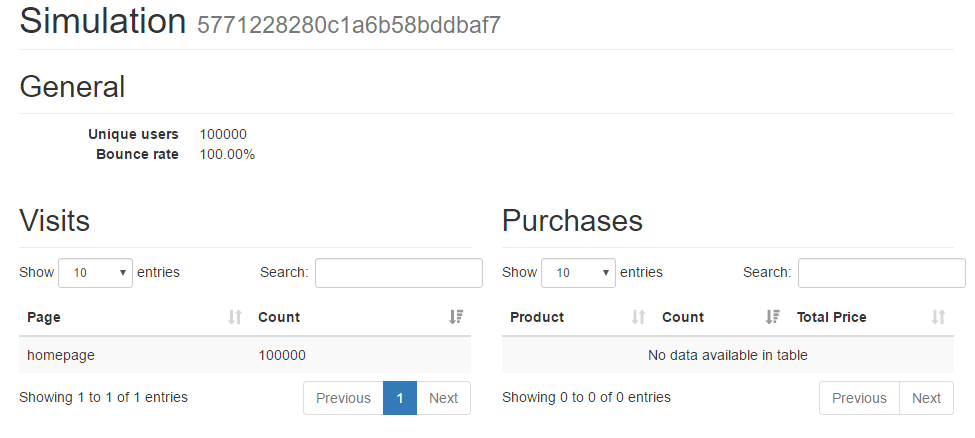
\includegraphics[width=1\textwidth]{expected_bounce_rate}
        \caption{Screenshot of the frontend results for this test run}
        \label{fig:test3result}
    \end{center}
\end{figure}

% \subsection{ test conversion rate, always buy -> 100% }

\section{Online store}

This test case uses data from a real online store that sells electronics and 
computers products. This website presents a fairly standard online store, 
mostly consisting of product listing and product pages. There are 3 places 
where it is possible to recommend products: the homepage has two sections, one 
with product highlights and another with product promotions and each product 
page has a tab to show related products.

\subsection{Input data and configuration}

The website consists of 2540 pages with 343201 links between pages, spanning 25 
base product categories and 103 sub-categories. There are 750 product list 
pages, 1748 product pages, 1 cart page and 41 uncategorised/generic pages, 
visualised in figure \ref{fig:cfcategories}.

\begin{figure}[h]
    \begin{center}
        \leavevmode
        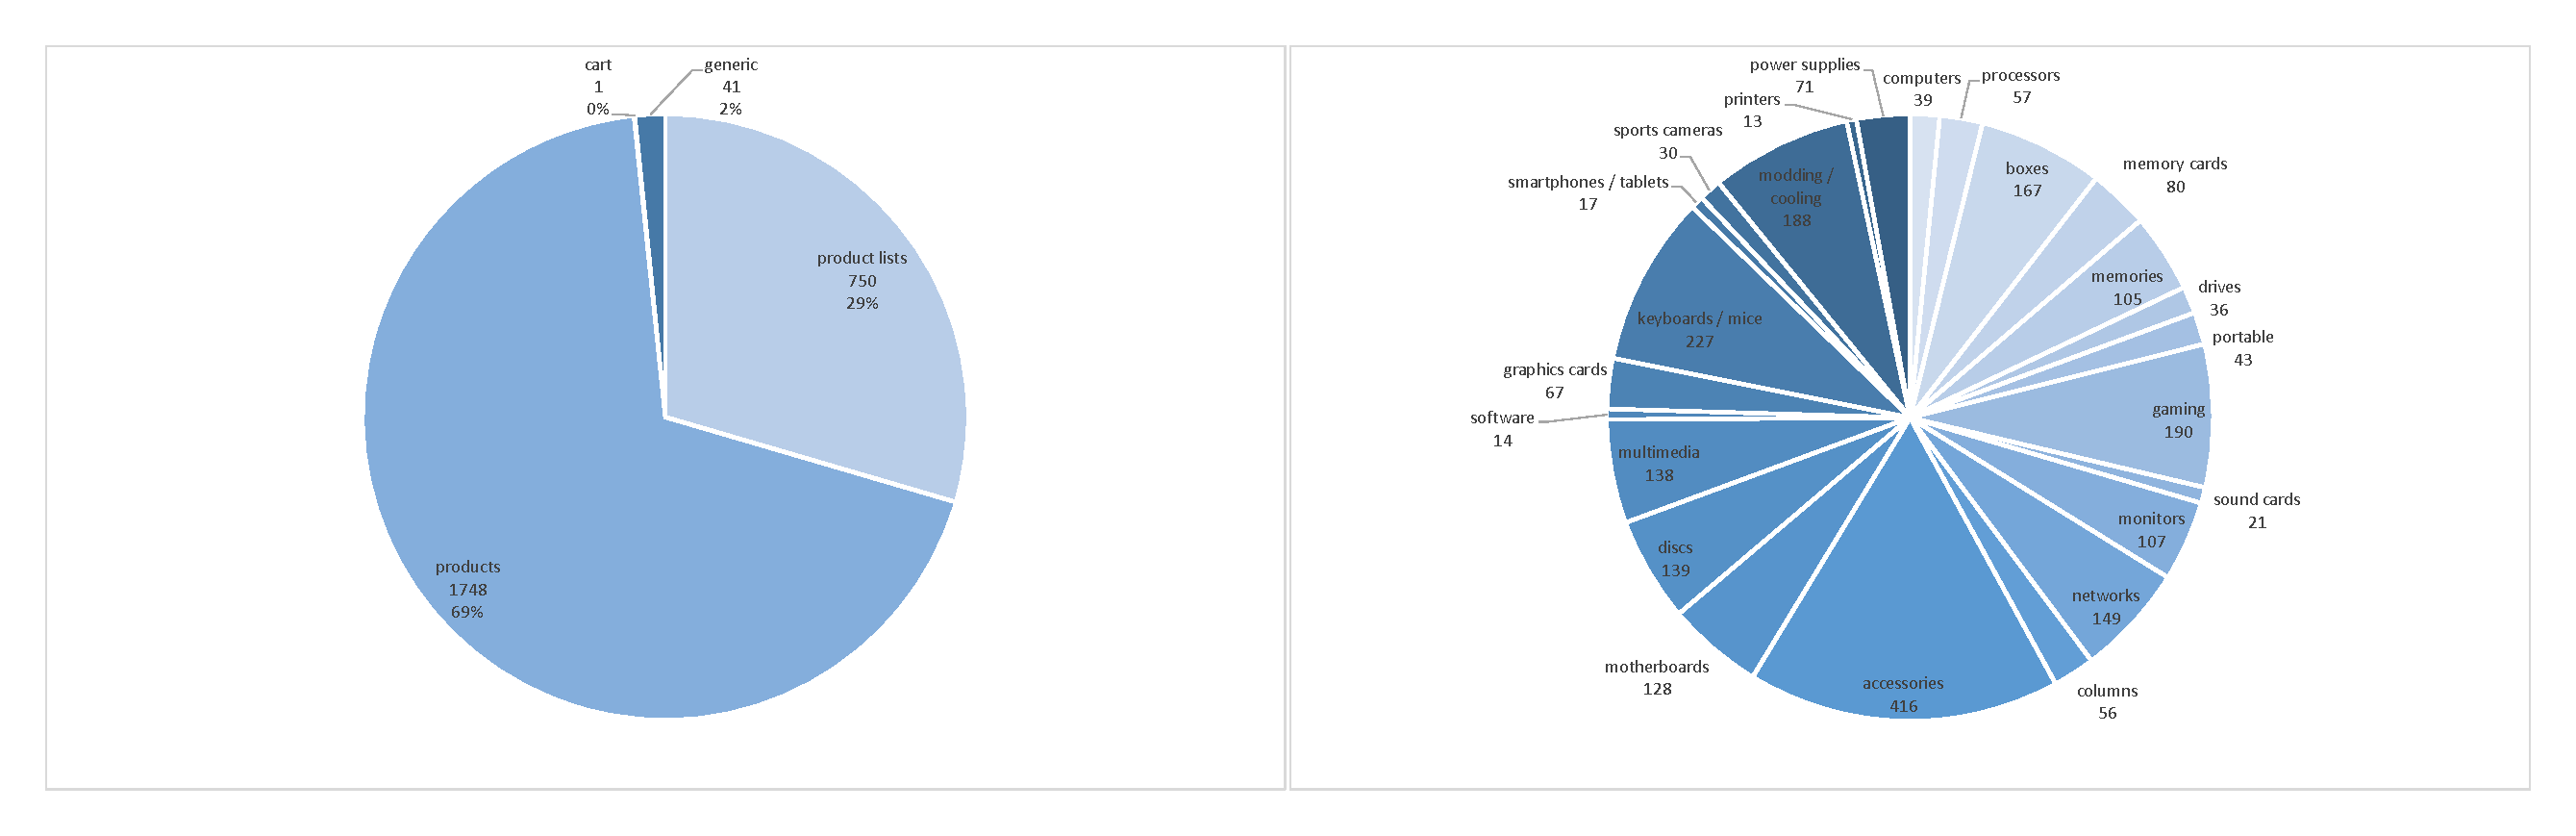
\includegraphics[width=1\textwidth]{cf_categories}
        \caption{Distribution of the type of pages in the website (left) and 
        distribution of the categories of the products (right)}
        \label{fig:cfcategories}
    \end{center}
\end{figure}

To simulate users and customers (the \texttt{NavigationAgent}s) interacting 
with this particular website, a model based on affinities was built. This model 
is composed by the \textit{affinities} themselves (a mapping between product 
categories and the likelihood of the user liking or having interest on products 
of that category), the probability of buying a product, the probability of 
exiting the website and the arrival rate.

Because real usage website data is not available for this website, a sample 
profile was created with the following properties: the affinities were set up 
as displayed in table \ref{tab:sample_user}, probability of buying set to 
$5\%$, probability of leaving the website of $15\%$ and a rate of arrival to 
the website following a \textit{Poisson} distribution with $\lambda = 500$.

\begin{table}[h]
    \centering
    \caption{Affinities for a sample user}
    \label{tab:sample_user}
    \begin{tabular}{@{}ll@{}}
        \toprule
        \textbf{Category}  & \textbf{Weight}  \\ \midrule
        Computadores       & 14.29\% \\
        MSI                & 14.29\% \\
        Pen Drives         & 7.14\%  \\
        Portáteis          & 14.29\% \\
        Intel 2011         & 14.29\% \\
        Cartões de Memória & 7.14\%  \\
        Brand              & 14.29\% \\
        Processadores      & 14.29\% \\ \bottomrule
    \end{tabular}
\end{table}

\subsection{Simulation}

The simulation was configured as described in the subsection above. All the 
navigation agents use the same profile. The "thought" process for each agent is 
fairly simple: at each step, they try to buy a product and exit the website in 
accordance to the probabilities defined \textit{a priori} or navigate to a 
different page based on their categories, with preference as stated by the 
affinity table. The simulation was run for 30 steps.

\subsection{Results}

The results of a sample simulation run are summarized in the tables 
\ref{tab:visitscat} and \ref{tab:genstats}. They are expected: the number of 
unique users is 14894 and the expected value is 15000 ($500 \times 25$); the 
bounce rate is $14.58\%$ and the prior leaving rate is $15\%$; and the 
conversion rate is $4.77\%$ and the prior buy rate is $5\%$.

\begin{table}[h]
    \centering
    \caption{Visits per category for a sample simulation run}
    \label{tab:visitscat}
    \begin{tabular}{@{}lll@{}}
        \toprule
        \textbf{Category}                   & \textbf{Sub-category} & 
        \textbf{Count} \\ \midrule
        \multirow{5}{*}{Cartões de Memória} & Pen Drives            & 
        6492           \\
        & SD/MiniSD/MicroSD     & 1203           \\
        & Leitor de Cartões     & 1199           \\
        & Compact Flash         & 1158           \\
        & -                     & 37             \\ \midrule
        \multirow{4}{*}{Portáteis}          & MSI                   & 
        14326          \\
        & HP                    & 2623           \\
        & Asus                  & 2584           \\
        & -                     & 263            \\ \midrule
        \multirow{5}{*}{Processadores}      & Intel 2011            & 
        7097           \\
        & Intel 1151            & 2752           \\
        & Intel 1150            & 2379           \\
        & AMD                   & 2234           \\
        & -                     & 240            \\ \midrule
        \multirow{2}{*}{Computadores}       & Brand                 & 
        19802          \\
        & -                     & 188            \\ \midrule
        Motherboards                        & Intel 2011            & 
        4917           \\ \bottomrule
    \end{tabular}
\end{table}

\begin{table}[h]
    \centering
    \caption{Metrics/info regarding a sample simulation run}
    \label{tab:genstats}
    \begin{tabular}{@{}ll@{}}
        \toprule
        \textbf{Field}  & \textbf{Value}               \\ \midrule
        Unique users    & 14894                        \\
        Bounce rate     & 14.58\%                      \\
        Conversion rate & 4.77\%                       \\
        Purchases       & 676                          \\
        NavAgentFactory & AffinityFactory              \\
        NavAgent        & AffinityUser                 \\
        WebsiteAgent    & DummyWebsiteAgent            \\
        Start time      & Thu Jul 07 14:14:36 BST 2016 \\
        End time        & Thu Jul 07 14:14:39 BST 2016 \\ \bottomrule
    \end{tabular}
\end{table}

%\section{Comparison shopping website}

%\todo{...}

%\subsection{Input data and configuration}
%\subsection{Simulation}
%\subsection{Results}
 % state of the art: models
\chapter{Methodology}\label{chap:method}

\section*{}

In this chapter we intend to describe the methodology to be followed on this 
dissertation and propose a work plan.

% Este capítulo deve começar por fazer uma apresentação detalhada do
%problema a resolver\footnote{Na introdução a apresentação do
%  problema foi breve.} podendo mesmo, caso se justifique,
%constituir-se um capítulo com essa finalidade.
 
%Deve depois dedicar-se à apresentação da solução sem detalhes de
%implementação. 
%Dependendo do trabalho, pode ser uma descrição mais teórica, mais
%``arquitetural'', etc.

\section{Methodology} \label{sec:meth}

Like any software development project, a simulation project also has a life 
cycle. In this section we describe the steps to apply in the simulation 
methodology, based on Ulgen et al.~\cite{Ulgen1994} and Banks et 
al.~\cite[section 1.11]{Banks2004}, which can be summarized as follows:

\begin{enumerate}
    \item \textit{Problem formulation}: Clear statement of the problem by the 
    analyst and stakeholders; \label{enum:mform}
    \item \textit{Setting of objectives and overall project plan}: Questions to 
    be answered by the simulation, plans for the study, cost and number of days 
    for each phase, with the results expected at each stage; \label{enum:mobj}
    \item \textit{Model conceptualization}: Select, modify and iterate over the 
    assumptions that characterize the system; \label{enum:mconcept}
    \item \textit{Data collection}: Collect the necessary data to run and 
    validate the model, assuming that required data will change with the 
    increasing complexity of the system; \label{enum:mdata}
    \item \textit{Model translation}: Materialization of the system in a 
    program; \label{enum:mtransl}
    \item \textit{Verification}: Making sure that the program behaves correctly 
    accordingly to its inputs; \label{enum:mverif}
    \item \textit{Validation}: Calibration of the model, comparing the model 
    against an actual system; \label{enum:mvalid}
    \item \textit{Experimental design}: Tweak the experiments, comparing 
    alternative designs; \label{enum:mexp}
    \item \textit{Production runs and analysis}: Estimate measures of 
    performance for the systems that are being simulated; \label{enum:mprod}
    \item \textit{Documentation and reporting}: Document both the program and 
    the progress of the study; \label{enum:mdocs}
    \item \textit{Implementation}: End result of the study, including the 
    entire simulation process. \label{enum:mimpl}
\end{enumerate}

This process can be visualized in figure \ref{fig:sim}.

\begin{figure}[h]
    \begin{center}
        \leavevmode
        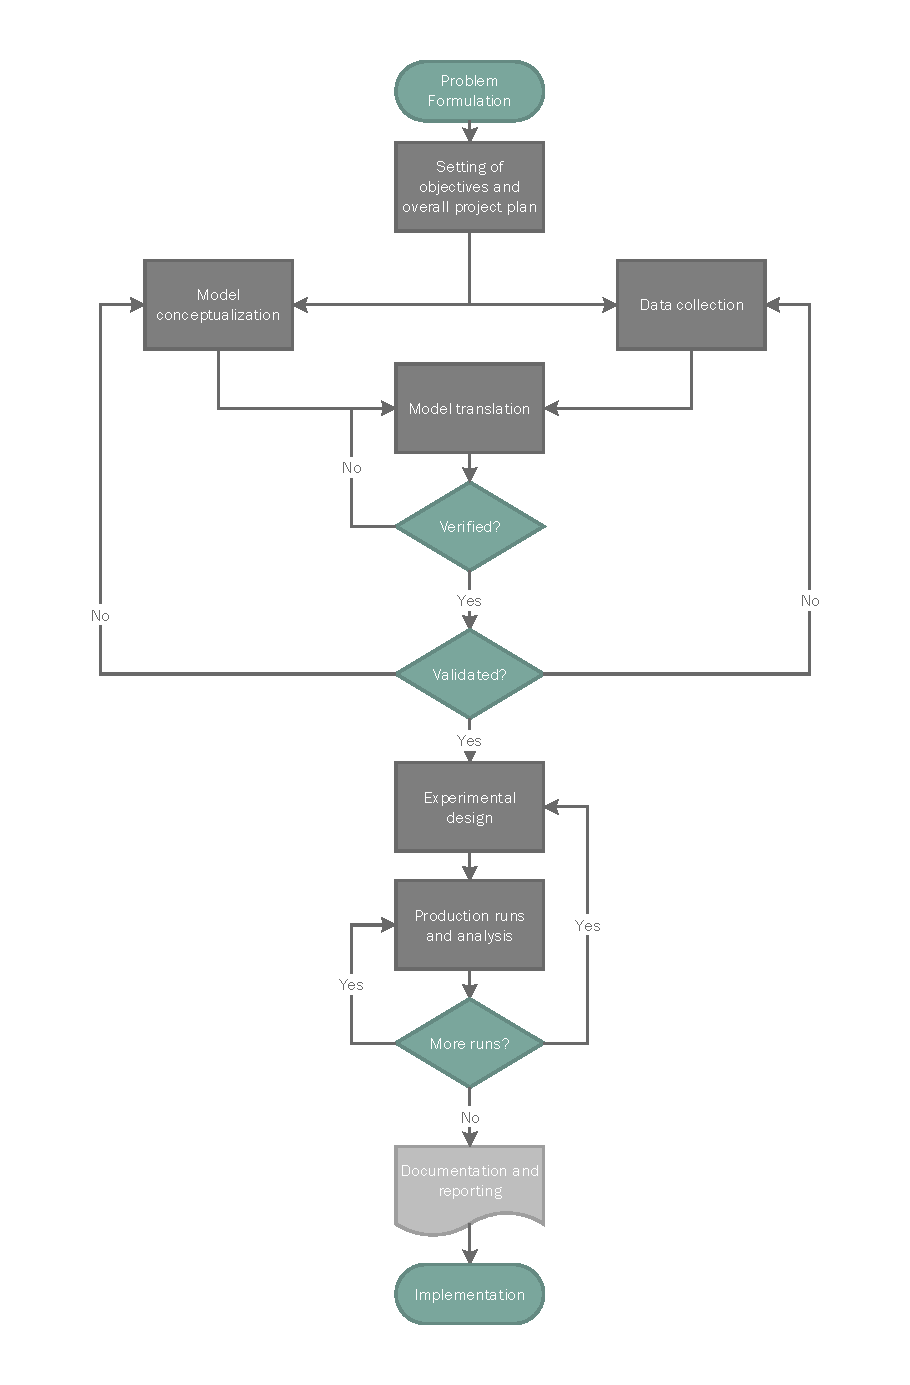
\includegraphics[width=0.6\textwidth]{simulation_study}
        \caption{Steps in a simulation study \cite{Banks2004}}
        \label{fig:sim}
    \end{center}
\end{figure}

\section{Planning}

Taking into account the steps described in section \ref{sec:meth}, a Gantt 
diagram was developed to define the tasks and their duration. This diagram is 
shown in appendix \ref{ap1:work_plan}.

We now present the details of the most important planned tasks. The name scheme 
follows \cite{Banks2004}.

\subsection{Discovery}

\begin{itemize}
    \item \textbf{Description}: Consists of the steps \textit{Problem 
    formulation} (\ref{enum:mform}) and \textit{Setting of objectives and 
    overall project plan} (\ref{enum:mobj}) presented above. In this stage the 
    initial statement of the problem and objectives are fine-tuned and 
    clarified.
    \item \textbf{Input}: Literature review on simulation, e-commerce and user 
    behaviour modelling and reunions with the supervisor.
    \item \textbf{Result}: Further clarification on the problem, overview and 
    analysis of the literature related with the dissertation and this report.
    \item \textbf{Time frame}: 01/10/2015 - 19/02/2016 (~20 weeks).
\end{itemize}

\subsection{Model building and data collection}

\begin{itemize}
    \item \textbf{Description}: Corresponds to the steps \ref{enum:mconcept} 
    to \ref{enum:mvalid} presented above. In this stage, the fundamental part 
    of the work is done and iterated multiple times. Emphasis should be given 
    to the reproducibility and validation of the process. This stage will be 
    further detailed during the dissertation period.
    \item \textbf{Input}: This report.
    \item \textbf{Result}: Runnable and testable simulation system, accompanied 
    by plausible scenarios (data) to feed the simulation.
    \item \textbf{Time frame}: 22/02/2016 - 15/04/2016 (~8 weeks).
\end{itemize}

\subsection{Running the model}

\begin{itemize}
    \item \textbf{Description}: Involves the steps \textit{Experimental design} 
    (\ref{enum:mexp}) and \textit{Production runs and analysis} 
    (\ref{enum:mprod}). In this stage, the model/system is tweaked and 
    statistical analysis is done on the experiment results.
    \item \textbf{Input}: Runnable simulation system.
    \item \textbf{Result}: Measurements of performance of the system being 
    evaluated.
    \item \textbf{Time frame}: 18/04/2016 - 06/05/2016 (~3 weeks).
\end{itemize}

\subsection{Implementation}

\begin{itemize}
    \item \textbf{Description}: Includes the steps \textit{Documentation and 
    reporting} (\ref{enum:mdocs}) and \textit{Implementation} 
    (\ref{enum:mimpl}). This final stage should conclude the dissertation, by 
    delivering the implementation of the framework/simulation engine and the 
    final dissertation report.
    \item \textbf{Input}: All the deliverables produced up to this point.
    \item \textbf{Result}: Documentation, dissertation report, concrete 
    simulation system implementation and verifiable results.
    \item \textbf{Time frame}: 09/05/2016 - 04/07/2016 (~8 weeks).
\end{itemize}

Architecture of the solution, implementation details (e.g. technologies) and on 
what actually consists a \textit{framework} were purposely left out of this 
planning dissertation report.
 % problem & solution
\chapter{Conclusion} \label{chap:conclusion}

\section*{}

This chapter concludes the work realized for the dissertation planning. It 
presents the conclusions including a SWOT analysis.

\section{Conclusion}

The state of the art literature review focused on three main areas, e-commerce, 
simulation and probabilistic models. There was an attempt at showing the 
classic techniques and approaches but also in showing extensions and 
improvements to those.

In order to better assess the work required for the dissertation, a SWOT 
analysis is in order.

\subsection{SWOT Analysis}

Regarding strengths, there is a wide and vast research in the area of 
simulation and modelling. There is also a strong confidence that the methods, 
approaches and techniques reviewed in the state of the art can be used to model 
user browsing behaviour successfully.

Concerning weaknesses, the proposed framework relates to many different areas, 
which may make the dissertation too broad in scope, making it hard to focus on 
something specific (``do one thing and do it well''\footnote{Unix philosophy}).

In regards to opportunities, no other similar framework or tool was found, 
which means that the work being done might be novel and may provide extra value 
to third parties (e.g the scientific community as tool to validate and test 
others models like recommendation systems or to companies focusing on 
e-commerce).

Regarding threats, testing and validating the framework may be problematic, in 
terms of corroborating results with real data or even finding a suitable 
approach to validation itself.
 % conclusion & future work

%%----------------------------------------
%% Final materials 
%%----------------------------------------

%% Bibliography
%% Comment the next command if BibTeX file not used
%% bibliography is in ``myrefs.bib''
\PrintBib{myrefs}

%% comment next 2 commands if numbered appendices are not used
\appendix
\chapter{Graphical User Interface} \label{ap1:interface} % rename

The following images are screenshots of the interface developed to visualize 
simulation runs.

\begin{figure}
    \begin{center}
        \leavevmode
        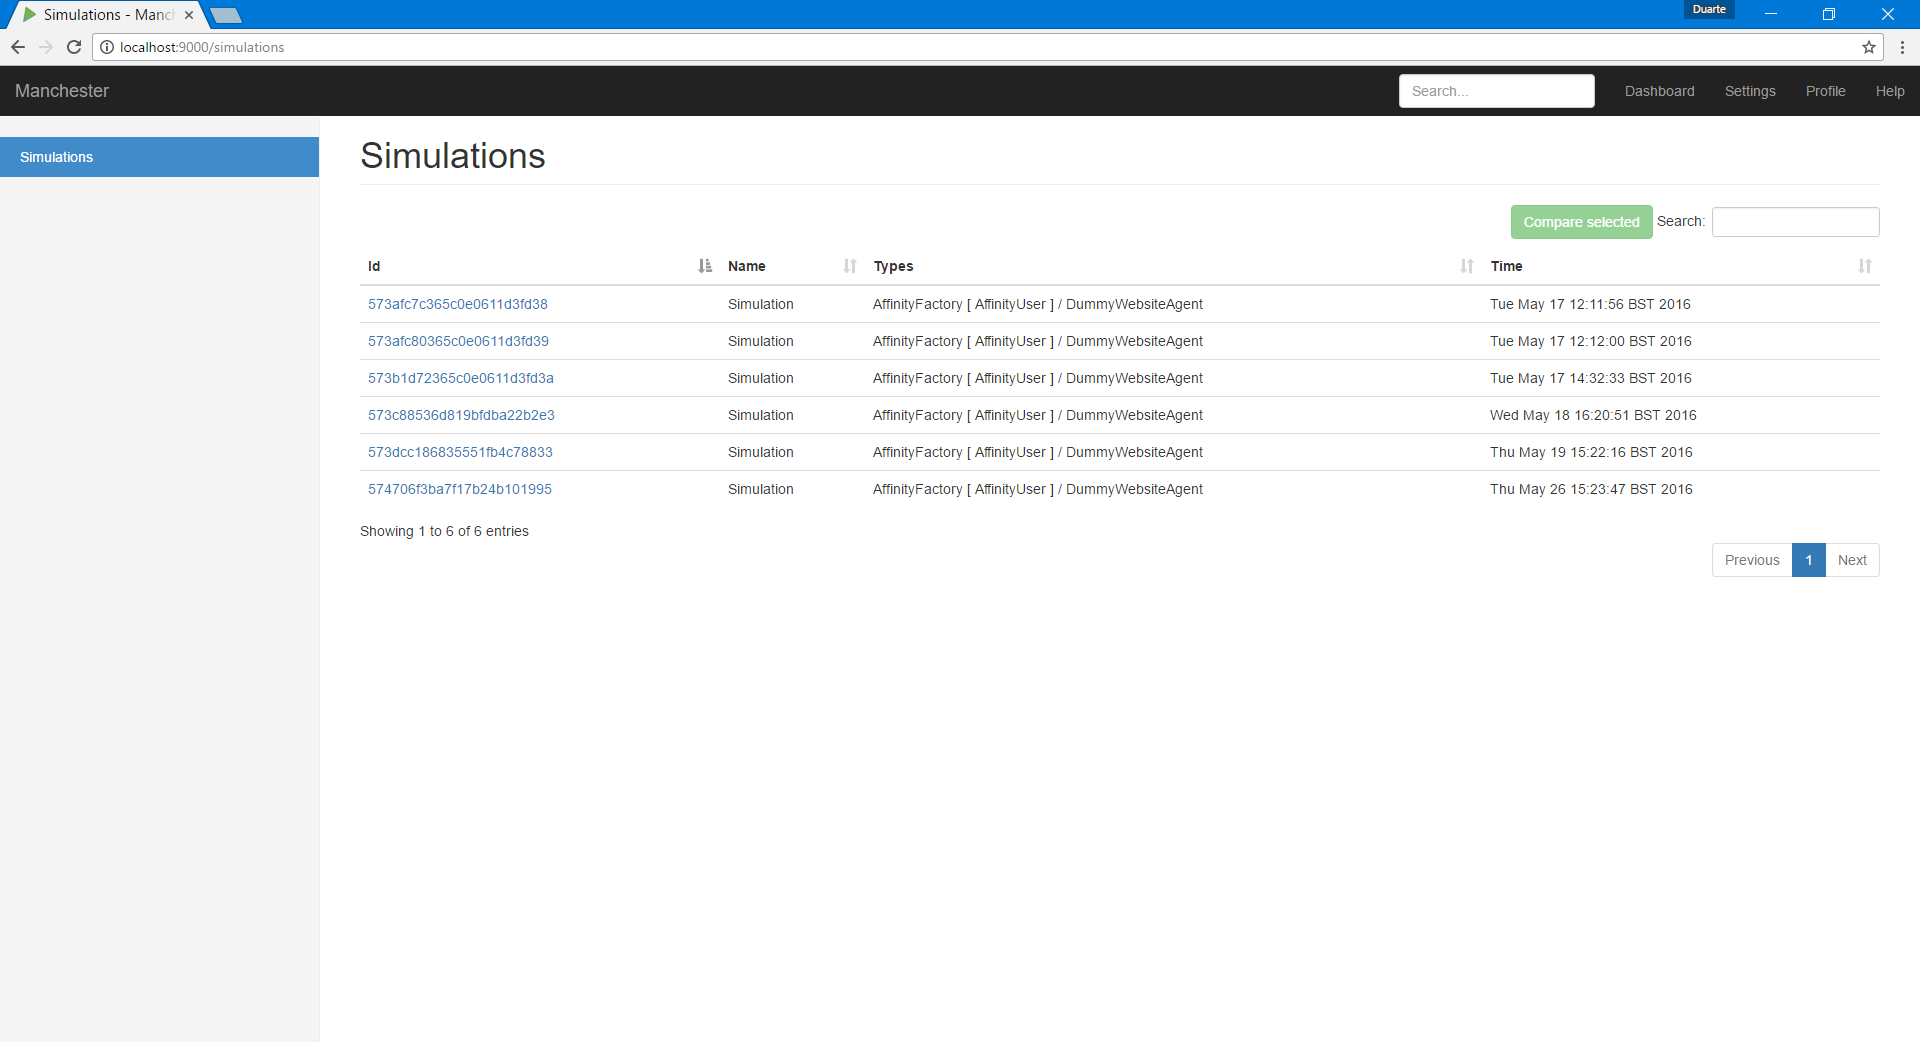
\includegraphics[width=1\textwidth]{sim_view}
        \caption{Screenshot of the simulations list page}
        \label{fig:sim_view}
    \end{center}
\end{figure}

\begin{figure}[p]
    \begin{center}
        \leavevmode
        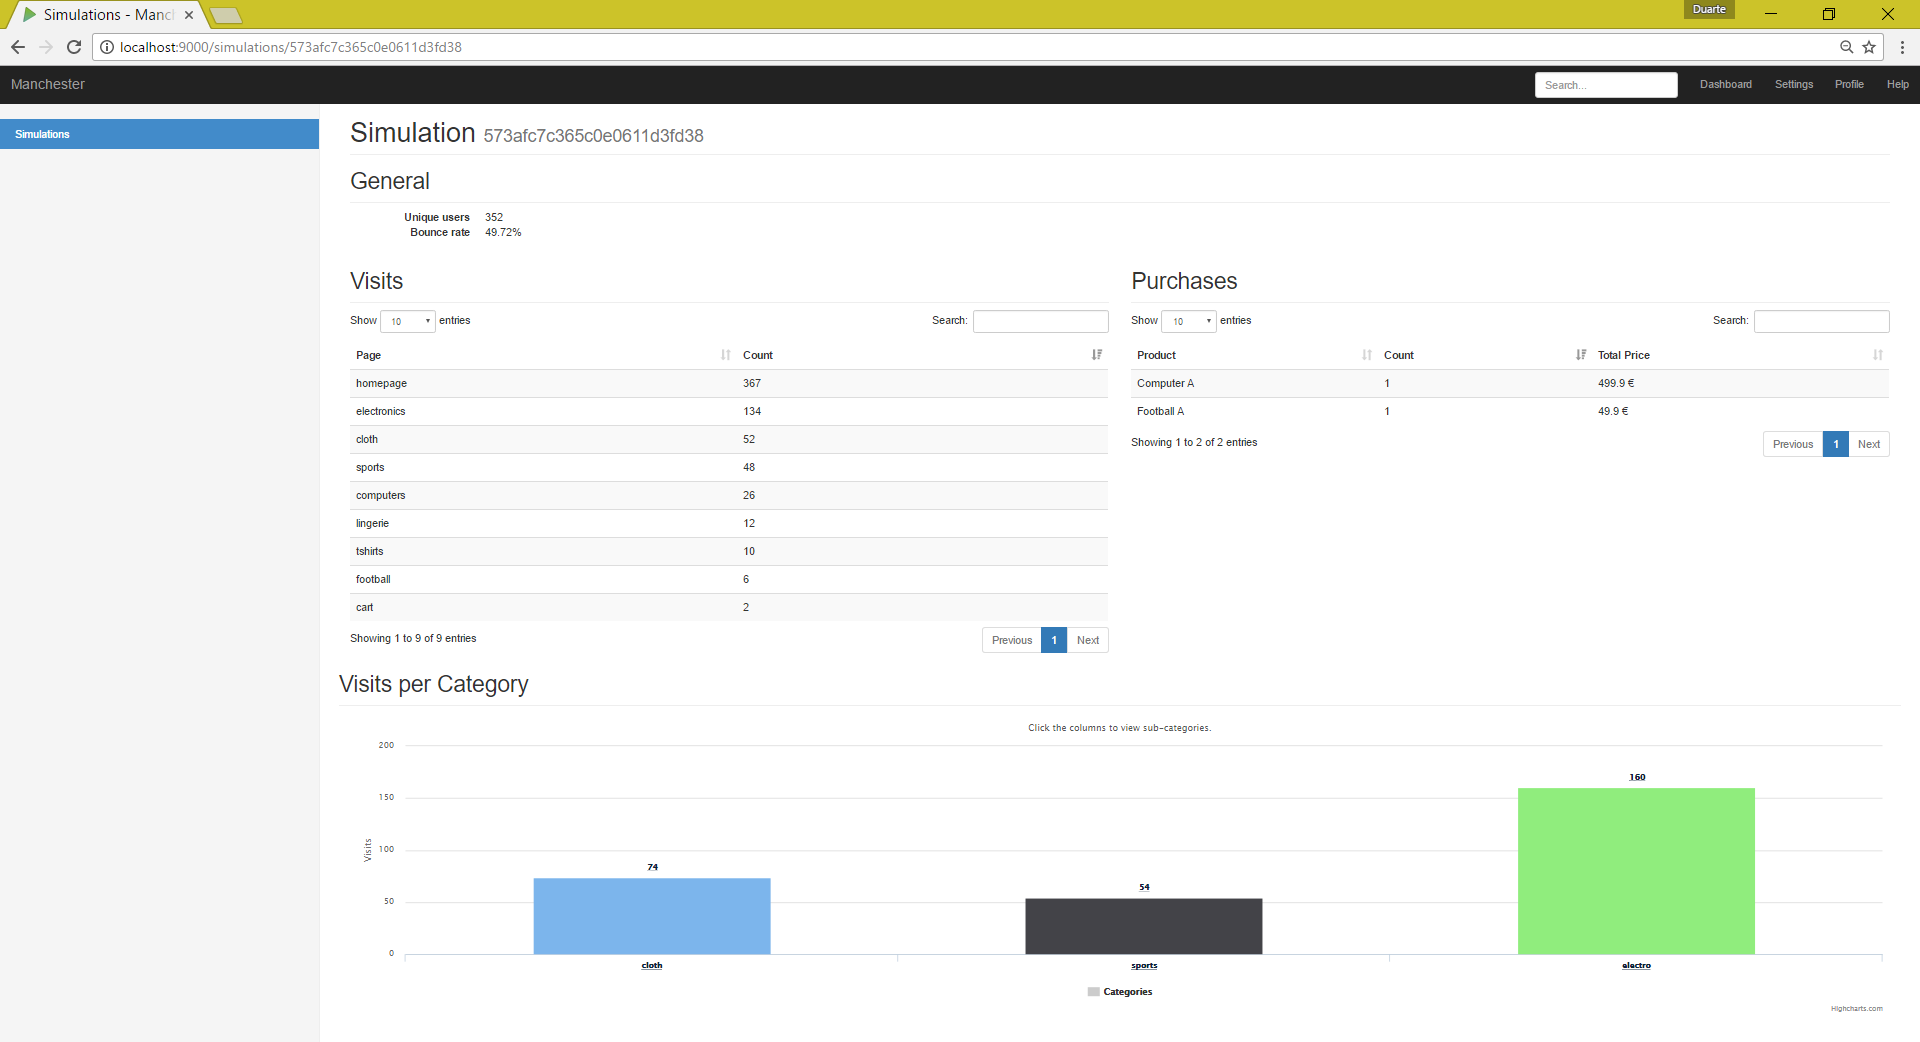
\includegraphics[width=1\textwidth]{sim_detail_view}
        \caption{Screenshot of the simulation detail page}
        \label{fig:sim_detail_view}
    \end{center}
\end{figure}

\begin{figure}[p]
    \begin{center}
        \leavevmode
        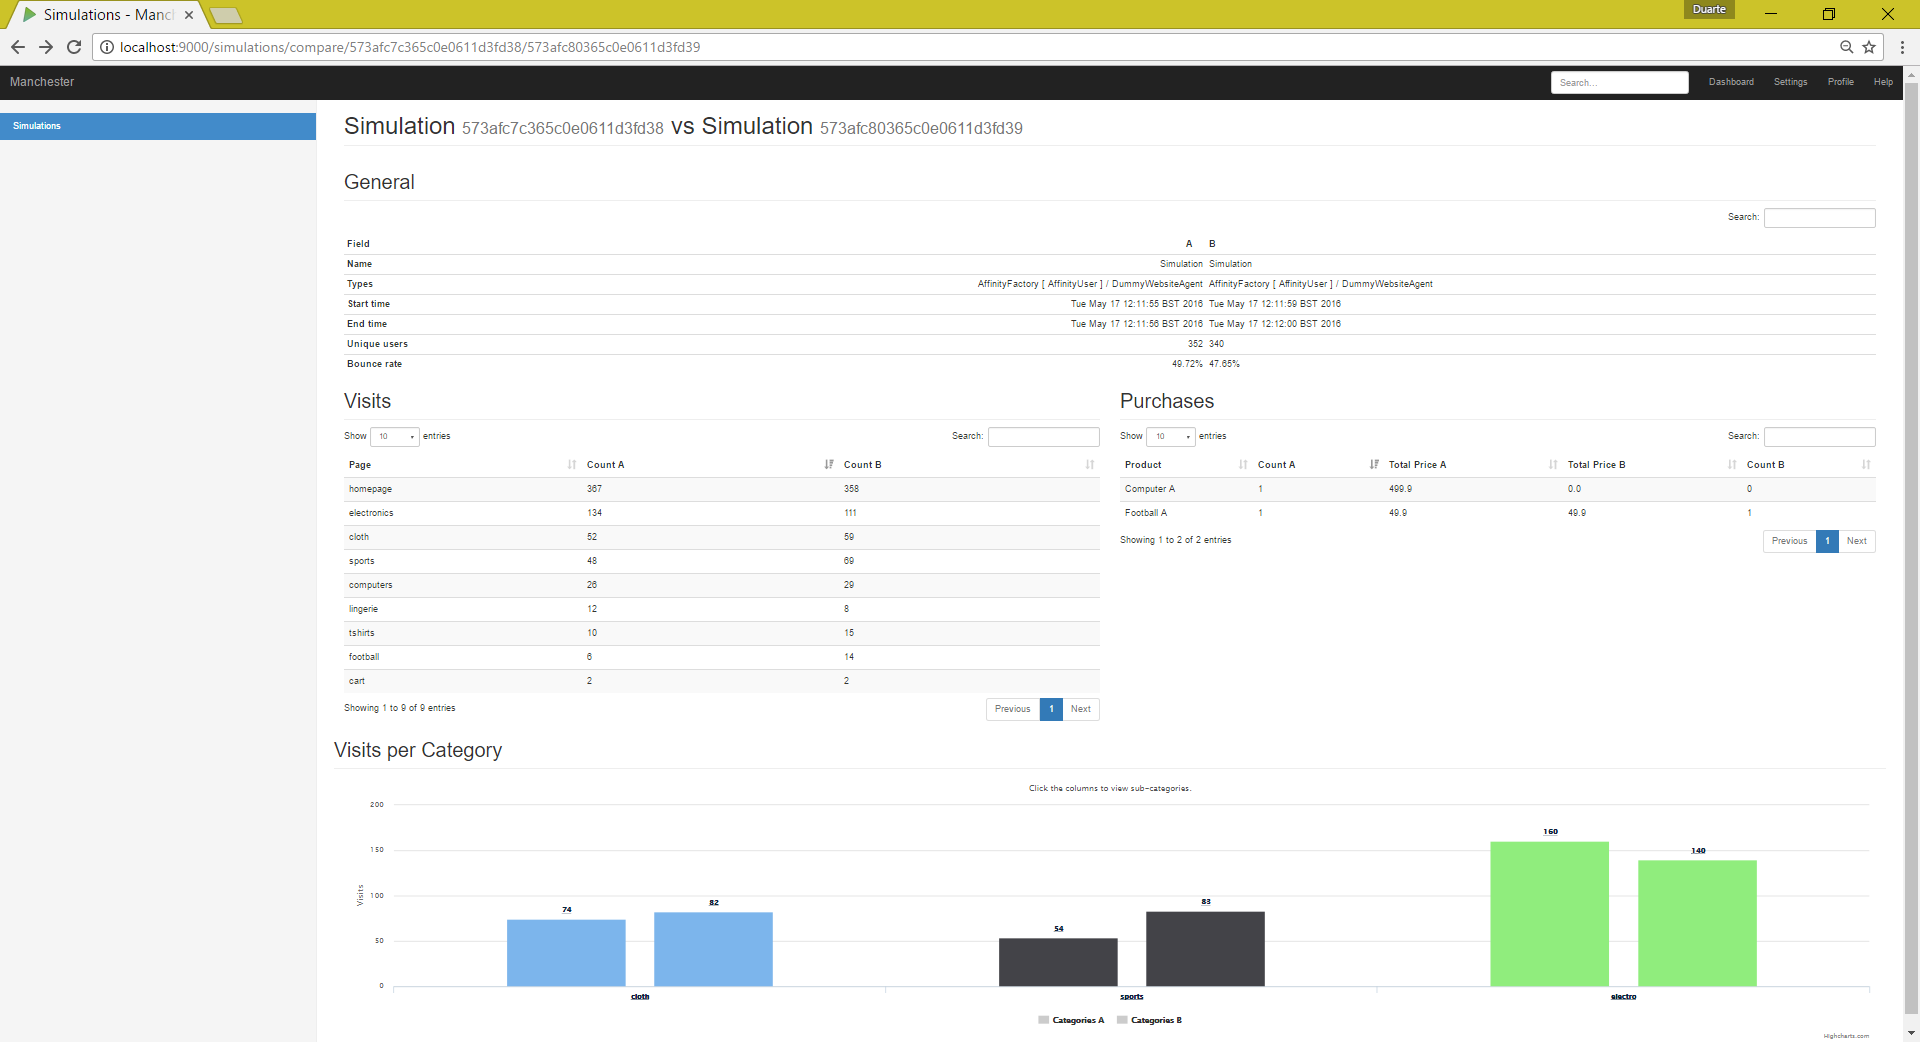
\includegraphics[width=1\textwidth]{sim_compare_view}
        \caption{Screenshot of the simulation comparison view}
        \label{fig:sim_compare_view}
    \end{center}
\end{figure}

%\begin{sidewaysfigure}
%	\centering
%	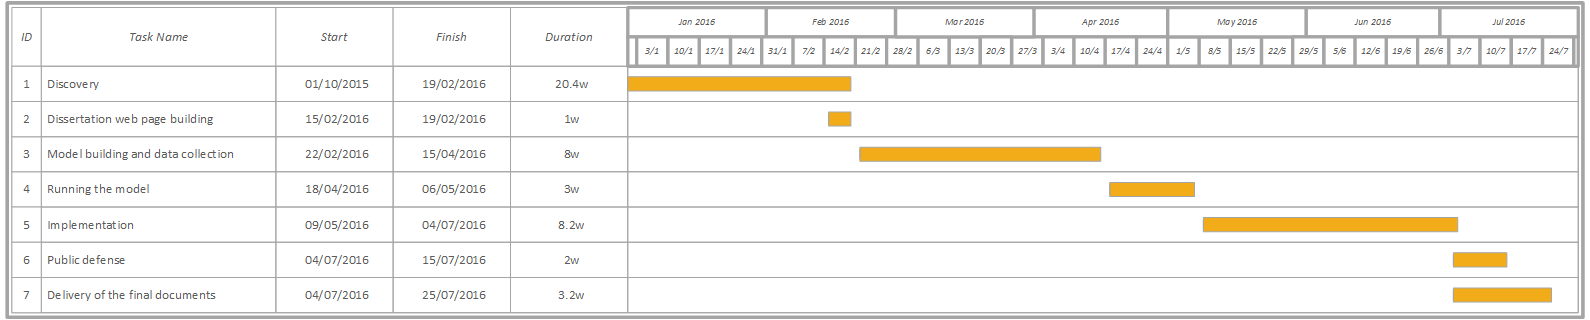
\includegraphics[width=0.86\textwidth]{thesis_gantt_chart}
%	\caption{Gantt Diagram}
%	\label{fig:gantt}
%\end{sidewaysfigure}


%% Index
%% Uncomment next command if index is required
%% don't forget to run ``makeindex mieic-en'' command
%\PrintIndex

\end{document}
